% Options for packages loaded elsewhere
\PassOptionsToPackage{unicode}{hyperref}
\PassOptionsToPackage{hyphens}{url}
%
\documentclass[
]{article}
\usepackage{amsmath,amssymb}
\usepackage{iftex}
\ifPDFTeX
  \usepackage[T1]{fontenc}
  \usepackage[utf8]{inputenc}
  \usepackage{textcomp} % provide euro and other symbols
\else % if luatex or xetex
  \usepackage{unicode-math} % this also loads fontspec
  \defaultfontfeatures{Scale=MatchLowercase}
  \defaultfontfeatures[\rmfamily]{Ligatures=TeX,Scale=1}
\fi
\usepackage{lmodern}
\ifPDFTeX\else
  % xetex/luatex font selection
\fi
% Use upquote if available, for straight quotes in verbatim environments
\IfFileExists{upquote.sty}{\usepackage{upquote}}{}
\IfFileExists{microtype.sty}{% use microtype if available
  \usepackage[]{microtype}
  \UseMicrotypeSet[protrusion]{basicmath} % disable protrusion for tt fonts
}{}
\makeatletter
\@ifundefined{KOMAClassName}{% if non-KOMA class
  \IfFileExists{parskip.sty}{%
    \usepackage{parskip}
  }{% else
    \setlength{\parindent}{0pt}
    \setlength{\parskip}{6pt plus 2pt minus 1pt}}
}{% if KOMA class
  \KOMAoptions{parskip=half}}
\makeatother
\usepackage{xcolor}
\usepackage[margin=1in]{geometry}
\usepackage{color}
\usepackage{fancyvrb}
\newcommand{\VerbBar}{|}
\newcommand{\VERB}{\Verb[commandchars=\\\{\}]}
\DefineVerbatimEnvironment{Highlighting}{Verbatim}{commandchars=\\\{\}}
% Add ',fontsize=\small' for more characters per line
\usepackage{framed}
\definecolor{shadecolor}{RGB}{248,248,248}
\newenvironment{Shaded}{\begin{snugshade}}{\end{snugshade}}
\newcommand{\AlertTok}[1]{\textcolor[rgb]{0.94,0.16,0.16}{#1}}
\newcommand{\AnnotationTok}[1]{\textcolor[rgb]{0.56,0.35,0.01}{\textbf{\textit{#1}}}}
\newcommand{\AttributeTok}[1]{\textcolor[rgb]{0.13,0.29,0.53}{#1}}
\newcommand{\BaseNTok}[1]{\textcolor[rgb]{0.00,0.00,0.81}{#1}}
\newcommand{\BuiltInTok}[1]{#1}
\newcommand{\CharTok}[1]{\textcolor[rgb]{0.31,0.60,0.02}{#1}}
\newcommand{\CommentTok}[1]{\textcolor[rgb]{0.56,0.35,0.01}{\textit{#1}}}
\newcommand{\CommentVarTok}[1]{\textcolor[rgb]{0.56,0.35,0.01}{\textbf{\textit{#1}}}}
\newcommand{\ConstantTok}[1]{\textcolor[rgb]{0.56,0.35,0.01}{#1}}
\newcommand{\ControlFlowTok}[1]{\textcolor[rgb]{0.13,0.29,0.53}{\textbf{#1}}}
\newcommand{\DataTypeTok}[1]{\textcolor[rgb]{0.13,0.29,0.53}{#1}}
\newcommand{\DecValTok}[1]{\textcolor[rgb]{0.00,0.00,0.81}{#1}}
\newcommand{\DocumentationTok}[1]{\textcolor[rgb]{0.56,0.35,0.01}{\textbf{\textit{#1}}}}
\newcommand{\ErrorTok}[1]{\textcolor[rgb]{0.64,0.00,0.00}{\textbf{#1}}}
\newcommand{\ExtensionTok}[1]{#1}
\newcommand{\FloatTok}[1]{\textcolor[rgb]{0.00,0.00,0.81}{#1}}
\newcommand{\FunctionTok}[1]{\textcolor[rgb]{0.13,0.29,0.53}{\textbf{#1}}}
\newcommand{\ImportTok}[1]{#1}
\newcommand{\InformationTok}[1]{\textcolor[rgb]{0.56,0.35,0.01}{\textbf{\textit{#1}}}}
\newcommand{\KeywordTok}[1]{\textcolor[rgb]{0.13,0.29,0.53}{\textbf{#1}}}
\newcommand{\NormalTok}[1]{#1}
\newcommand{\OperatorTok}[1]{\textcolor[rgb]{0.81,0.36,0.00}{\textbf{#1}}}
\newcommand{\OtherTok}[1]{\textcolor[rgb]{0.56,0.35,0.01}{#1}}
\newcommand{\PreprocessorTok}[1]{\textcolor[rgb]{0.56,0.35,0.01}{\textit{#1}}}
\newcommand{\RegionMarkerTok}[1]{#1}
\newcommand{\SpecialCharTok}[1]{\textcolor[rgb]{0.81,0.36,0.00}{\textbf{#1}}}
\newcommand{\SpecialStringTok}[1]{\textcolor[rgb]{0.31,0.60,0.02}{#1}}
\newcommand{\StringTok}[1]{\textcolor[rgb]{0.31,0.60,0.02}{#1}}
\newcommand{\VariableTok}[1]{\textcolor[rgb]{0.00,0.00,0.00}{#1}}
\newcommand{\VerbatimStringTok}[1]{\textcolor[rgb]{0.31,0.60,0.02}{#1}}
\newcommand{\WarningTok}[1]{\textcolor[rgb]{0.56,0.35,0.01}{\textbf{\textit{#1}}}}
\usepackage{graphicx}
\makeatletter
\def\maxwidth{\ifdim\Gin@nat@width>\linewidth\linewidth\else\Gin@nat@width\fi}
\def\maxheight{\ifdim\Gin@nat@height>\textheight\textheight\else\Gin@nat@height\fi}
\makeatother
% Scale images if necessary, so that they will not overflow the page
% margins by default, and it is still possible to overwrite the defaults
% using explicit options in \includegraphics[width, height, ...]{}
\setkeys{Gin}{width=\maxwidth,height=\maxheight,keepaspectratio}
% Set default figure placement to htbp
\makeatletter
\def\fps@figure{htbp}
\makeatother
\setlength{\emergencystretch}{3em} % prevent overfull lines
\providecommand{\tightlist}{%
  \setlength{\itemsep}{0pt}\setlength{\parskip}{0pt}}
\setcounter{secnumdepth}{-\maxdimen} % remove section numbering
\ifLuaTeX
  \usepackage{selnolig}  % disable illegal ligatures
\fi
\IfFileExists{bookmark.sty}{\usepackage{bookmark}}{\usepackage{hyperref}}
\IfFileExists{xurl.sty}{\usepackage{xurl}}{} % add URL line breaks if available
\urlstyle{same}
\hypersetup{
  pdftitle={SIM Project 2. Model fitting},
  pdfauthor={Adrià Casanova Víctor Garcia Zhengyong Ji},
  hidelinks,
  pdfcreator={LaTeX via pandoc}}

\title{SIM Project 2. Model fitting}
\author{Adrià Casanova Víctor Garcia Zhengyong Ji}
\date{November, 19th 2023}

\begin{document}
\maketitle

{
\setcounter{tocdepth}{3}
\tableofcontents
}
To reduce the time of computations, we have split our code in two .Rmd
files. In this one, the preprocessed train dataset is found in df, while
the preprocessed test database is in df\_test.

\hypertarget{first-model-building}{%
\section{8. First model building}\label{first-model-building}}

We create a first model with all the numerical variables that we
selected previously.

\begin{Shaded}
\begin{Highlighting}[]
\NormalTok{df\_num }\OtherTok{\textless{}{-}}\NormalTok{ df[, }\FunctionTok{which}\NormalTok{(}\FunctionTok{sapply}\NormalTok{(df, is.numeric))]}
\NormalTok{m0 }\OtherTok{=} \FunctionTok{lm}\NormalTok{(SalePrice }\SpecialCharTok{\textasciitilde{}}\NormalTok{ ., }\AttributeTok{data=}\NormalTok{df\_num)}

\FunctionTok{summary}\NormalTok{(m0)}
\end{Highlighting}
\end{Shaded}

\begin{verbatim}
## 
## Call:
## lm(formula = SalePrice ~ ., data = df_num)
## 
## Residuals:
##     Min      1Q  Median      3Q     Max 
## -160830  -15890   -1092   14377  164012 
## 
## Coefficients:
##                Estimate Std. Error t value Pr(>|t|)    
## (Intercept)  -1.783e+06  1.122e+05 -15.887  < 2e-16 ***
## LotFrontage   8.821e+01  2.535e+01   3.480 0.000516 ***
## LotArea       1.508e+00  2.702e-01   5.581 2.86e-08 ***
## YearBuilt     4.597e+02  5.315e+01   8.650  < 2e-16 ***
## YearRemodAdd  5.492e+02  5.246e+01  10.469  < 2e-16 ***
## MasVnrArea    2.637e+01  6.338e+00   4.160 3.37e-05 ***
## BsmtFinSF1    1.975e+01  4.851e+00   4.072 4.91e-05 ***
## BsmtUnfSF     2.595e+00  4.872e+00   0.533 0.594302    
## TotalBsmtSF   3.133e+01  5.792e+00   5.408 7.45e-08 ***
## X1stFlrSF    -3.742e+01  1.263e+01  -2.964 0.003092 ** 
## X2ndFlrSF    -2.545e+01  1.219e+01  -2.087 0.037071 *  
## GrLivArea     9.523e+01  1.189e+01   8.008 2.40e-15 ***
## BsmtFullBath  5.513e+02  2.138e+03   0.258 0.796537    
## FullBath     -3.287e+03  2.399e+03  -1.370 0.170788    
## HalfBath     -3.521e+03  2.304e+03  -1.528 0.126693    
## BedroomAbvGr -1.013e+04  1.447e+03  -6.998 3.99e-12 ***
## TotRmsAbvGrd  4.475e+02  1.040e+03   0.430 0.667190    
## Fireplaces    8.700e+03  1.491e+03   5.836 6.59e-09 ***
## GarageYrBlt  -9.735e+01  6.592e+01  -1.477 0.139962    
## GarageCars    6.429e+03  2.464e+03   2.609 0.009169 ** 
## GarageArea    2.753e+01  8.866e+00   3.105 0.001943 ** 
## WoodDeckSF    2.326e+01  7.061e+00   3.294 0.001013 ** 
## OpenPorchSF   4.699e+01  1.561e+01   3.009 0.002664 ** 
## ---
## Signif. codes:  0 '***' 0.001 '**' 0.01 '*' 0.05 '.' 0.1 ' ' 1
## 
## Residual standard error: 29940 on 1425 degrees of freedom
## Multiple R-squared:  0.8233, Adjusted R-squared:  0.8206 
## F-statistic: 301.9 on 22 and 1425 DF,  p-value: < 2.2e-16
\end{verbatim}

\begin{Shaded}
\begin{Highlighting}[]
\FunctionTok{vif}\NormalTok{(m0)}
\end{Highlighting}
\end{Shaded}

\begin{verbatim}
##  LotFrontage      LotArea    YearBuilt YearRemodAdd   MasVnrArea   BsmtFinSF1 
##     1.141502     1.463022     4.139242     1.895906     1.313313     6.894967 
##    BsmtUnfSF  TotalBsmtSF    X1stFlrSF    X2ndFlrSF    GrLivArea BsmtFullBath 
##     7.381445     8.459562    33.083818    44.080849    53.497983     1.987127 
##     FullBath     HalfBath BedroomAbvGr TotRmsAbvGrd   Fireplaces  GarageYrBlt 
##     2.743664     2.161873     2.172081     4.340452     1.467970     4.270628 
##   GarageCars   GarageArea   WoodDeckSF  OpenPorchSF 
##     5.396088     5.481694     1.173485     1.223935
\end{verbatim}

There are a lot of features with a vif correlation larger than 5. So, in
order to reduce the amount of workload, we decided to keep those that
are less than 5 and are highly correlated with our target.

\begin{Shaded}
\begin{Highlighting}[]
\CommentTok{\# Let\textquotesingle{}s store the indices of the variables with at least one star in the lm and vif\textless{}5}
\NormalTok{id\_num\_star1 }\OtherTok{=} \FunctionTok{c}\NormalTok{(}\DecValTok{1}\SpecialCharTok{:}\DecValTok{5}\NormalTok{,}\DecValTok{15}\NormalTok{,}\DecValTok{17}\NormalTok{,}\DecValTok{21}\SpecialCharTok{:}\DecValTok{23}\NormalTok{)}
\NormalTok{df\_num1 }\OtherTok{\textless{}{-}}\NormalTok{ df\_num[, id\_num\_star1]}
\CommentTok{\# And build a new model only with significance features}
\NormalTok{m1 }\OtherTok{=} \FunctionTok{lm}\NormalTok{(SalePrice }\SpecialCharTok{\textasciitilde{}}\NormalTok{., }\AttributeTok{data=}\NormalTok{df\_num1)}
\FunctionTok{summary}\NormalTok{(m1)}
\end{Highlighting}
\end{Shaded}

\begin{verbatim}
## 
## Call:
## lm(formula = SalePrice ~ ., data = df_num1)
## 
## Residuals:
##     Min      1Q  Median      3Q     Max 
## -170973  -25349   -4048   18791  207331 
## 
## Coefficients:
##                Estimate Std. Error t value Pr(>|t|)    
## (Intercept)  -2.876e+06  1.159e+05 -24.820  < 2e-16 ***
## LotFrontage   1.951e+02  3.456e+01   5.645 1.99e-08 ***
## LotArea       3.960e+00  3.532e-01  11.212  < 2e-16 ***
## YearBuilt     5.558e+02  4.789e+01  11.607  < 2e-16 ***
## YearRemodAdd  9.359e+02  6.734e+01  13.897  < 2e-16 ***
## MasVnrArea    8.678e+01  8.411e+00  10.317  < 2e-16 ***
## BedroomAbvGr  5.492e+03  1.453e+03   3.781 0.000163 ***
## Fireplaces    2.779e+04  1.875e+03  14.826  < 2e-16 ***
## WoodDeckSF    5.749e+01  9.669e+00   5.946 3.44e-09 ***
## OpenPorchSF   1.478e+02  2.112e+01   6.997 4.00e-12 ***
## ---
## Signif. codes:  0 '***' 0.001 '**' 0.01 '*' 0.05 '.' 0.1 ' ' 1
## 
## Residual standard error: 41800 on 1438 degrees of freedom
## Multiple R-squared:  0.6525, Adjusted R-squared:  0.6503 
## F-statistic:   300 on 9 and 1438 DF,  p-value: < 2.2e-16
\end{verbatim}

\begin{Shaded}
\begin{Highlighting}[]
\FunctionTok{vif}\NormalTok{(m1)}
\end{Highlighting}
\end{Shaded}

\begin{verbatim}
##  LotFrontage      LotArea    YearBuilt YearRemodAdd   MasVnrArea BedroomAbvGr 
##     1.088404     1.282087     1.723739     1.602800     1.186320     1.122948 
##   Fireplaces   WoodDeckSF  OpenPorchSF 
##     1.190834     1.128839     1.149369
\end{verbatim}

\begin{Shaded}
\begin{Highlighting}[]
\CommentTok{\# As we can observe, vif correlations are much better, all values are less than 2.}
\CommentTok{\# So the next step is to check the correlation between predictors.}
\NormalTok{corr\_mat }\OtherTok{\textless{}{-}} \FunctionTok{cor}\NormalTok{(df\_num1)}
\FunctionTok{corrplot}\NormalTok{(corr\_mat, }\AttributeTok{method =} \StringTok{"number"}\NormalTok{)}
\end{Highlighting}
\end{Shaded}

\includegraphics{SIM-Project-2.-Model-Fitting_files/figure-latex/unnamed-chunk-5-1.pdf}

Feature ``YearBuilt'' and ``YearRemodAdd'' are highly correlated, and
``YearBuilt'' is more correlated to our target SalePrice. Hence, we
remove YearRemodAdd in the next model.

\begin{Shaded}
\begin{Highlighting}[]
\CommentTok{\# Building the model without "YearRemodAdd"}
\NormalTok{id\_num\_star2 }\OtherTok{=} \FunctionTok{c}\NormalTok{(}\DecValTok{1}\SpecialCharTok{:}\DecValTok{3}\NormalTok{,}\DecValTok{5}\NormalTok{,}\DecValTok{15}\NormalTok{,}\DecValTok{17}\NormalTok{,}\DecValTok{21}\SpecialCharTok{:}\DecValTok{23}\NormalTok{)}
\NormalTok{df\_num2 }\OtherTok{\textless{}{-}}\NormalTok{ df\_num[, id\_num\_star2]}
\NormalTok{m2 }\OtherTok{=} \FunctionTok{lm}\NormalTok{(SalePrice }\SpecialCharTok{\textasciitilde{}}\NormalTok{., }\AttributeTok{data=}\NormalTok{df\_num2)}
\FunctionTok{summary}\NormalTok{(m2)}
\end{Highlighting}
\end{Shaded}

\begin{verbatim}
## 
## Call:
## lm(formula = SalePrice ~ ., data = df_num2)
## 
## Residuals:
##     Min      1Q  Median      3Q     Max 
## -165690  -27970   -5057   19803  205977 
## 
## Coefficients:
##                Estimate Std. Error t value Pr(>|t|)    
## (Intercept)  -1.714e+06  8.539e+04 -20.069  < 2e-16 ***
## LotFrontage   2.282e+02  3.670e+01   6.218 6.59e-10 ***
## LotArea       3.810e+00  3.759e-01  10.136  < 2e-16 ***
## YearBuilt     9.075e+02  4.329e+01  20.966  < 2e-16 ***
## MasVnrArea    8.050e+01  8.942e+00   9.002  < 2e-16 ***
## BedroomAbvGr  5.014e+03  1.546e+03   3.243  0.00121 ** 
## Fireplaces    2.795e+04  1.996e+03  14.006  < 2e-16 ***
## WoodDeckSF    7.267e+01  1.023e+01   7.105 1.88e-12 ***
## OpenPorchSF   1.917e+02  2.224e+01   8.619  < 2e-16 ***
## ---
## Signif. codes:  0 '***' 0.001 '**' 0.01 '*' 0.05 '.' 0.1 ' ' 1
## 
## Residual standard error: 44500 on 1439 degrees of freedom
## Multiple R-squared:  0.6058, Adjusted R-squared:  0.6036 
## F-statistic: 276.4 on 8 and 1439 DF,  p-value: < 2.2e-16
\end{verbatim}

Now, the most correlated variables in our model have at most a
coefficient of correlation of 0.315, which in the context of real estate
it is weak. We have obtained this information from
\url{https://37parallel.com/real-estate-correlation/}.

\begin{Shaded}
\begin{Highlighting}[]
\FunctionTok{Anova}\NormalTok{(m2)}
\end{Highlighting}
\end{Shaded}

\begin{verbatim}
## Anova Table (Type II tests)
## 
## Response: SalePrice
##                  Sum Sq   Df F value    Pr(>F)    
## LotFrontage  7.6561e+10    1  38.662 6.588e-10 ***
## LotArea      2.0346e+11    1 102.744 < 2.2e-16 ***
## YearBuilt    8.7042e+11    1 439.553 < 2.2e-16 ***
## MasVnrArea   1.6047e+11    1  81.034 < 2.2e-16 ***
## BedroomAbvGr 2.0821e+10    1  10.515  0.001212 ** 
## Fireplaces   3.8845e+11    1 196.163 < 2.2e-16 ***
## WoodDeckSF   9.9972e+10    1  50.485 1.883e-12 ***
## OpenPorchSF  1.4712e+11    1  74.292 < 2.2e-16 ***
## Residuals    2.8496e+12 1439                      
## ---
## Signif. codes:  0 '***' 0.001 '**' 0.01 '*' 0.05 '.' 0.1 ' ' 1
\end{verbatim}

Anova shows that all the variables we have kept are relevant.

\hypertarget{model-analysis-and-iteration}{%
\section{9. Model analysis and
iteration}\label{model-analysis-and-iteration}}

First, let us plot the residuals of m2 to be able to compare them with
the next iterations of the model.

\begin{Shaded}
\begin{Highlighting}[]
\FunctionTok{par}\NormalTok{(}\AttributeTok{mfrow=}\FunctionTok{c}\NormalTok{(}\DecValTok{2}\NormalTok{,}\DecValTok{2}\NormalTok{))}
\FunctionTok{plot}\NormalTok{(m2)}
\end{Highlighting}
\end{Shaded}

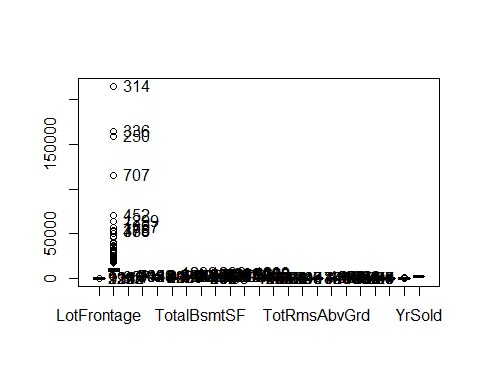
\includegraphics{SIM-Project-2.-Model-Fitting_files/figure-latex/unnamed-chunk-8-1.pdf}

We analysed if there were influential data and found 3 observations with
a bigger Cook's distance than the threshold (considered as 2/sqrt(n)).
Consequently, we decided to remove those observations.

\begin{Shaded}
\begin{Highlighting}[]
\CommentTok{\# Check the influential plot before removing the influential observation.}
\FunctionTok{influencePlot}\NormalTok{(m2)}
\end{Highlighting}
\end{Shaded}

\includegraphics{SIM-Project-2.-Model-Fitting_files/figure-latex/unnamed-chunk-9-1.pdf}

\begin{verbatim}
##         StudRes         Hat        CookD
## 54    4.4351943 0.011705638 2.555600e-02
## 494   4.6798339 0.007521628 1.817802e-02
## 662   2.9293234 0.027500038 2.681970e-02
## 1260  0.9231784 0.034051251 3.338507e-03
## 1412 -0.1455309 0.030239831 7.343087e-05
\end{verbatim}

\begin{Shaded}
\begin{Highlighting}[]
\CommentTok{\# Calculate D\textquotesingle{}s threshold}
\NormalTok{D\_thresh }\OtherTok{\textless{}{-}} \DecValTok{2}\SpecialCharTok{/}\FunctionTok{sqrt}\NormalTok{(}\FunctionTok{dim}\NormalTok{(df\_num2)[}\DecValTok{1}\NormalTok{]); D\_thresh}
\end{Highlighting}
\end{Shaded}

\begin{verbatim}
## [1] 0.05255883
\end{verbatim}

\begin{Shaded}
\begin{Highlighting}[]
\CommentTok{\#Remove the points and fit the model again}
\NormalTok{influent }\OtherTok{\textless{}{-}} \FunctionTok{c}\NormalTok{(}\DecValTok{1183}\NormalTok{, }\DecValTok{692}\NormalTok{, }\DecValTok{186}\NormalTok{)}

\NormalTok{df }\OtherTok{\textless{}{-}}\NormalTok{ df[}\SpecialCharTok{{-}}\NormalTok{influent,]}
\NormalTok{df\_num }\OtherTok{\textless{}{-}}\NormalTok{ df[, }\FunctionTok{which}\NormalTok{(}\FunctionTok{sapply}\NormalTok{(df, is.numeric))]}
\NormalTok{df\_num2 }\OtherTok{\textless{}{-}}\NormalTok{ df\_num[, id\_num\_star2]}
\NormalTok{m2 }\OtherTok{=} \FunctionTok{lm}\NormalTok{(SalePrice }\SpecialCharTok{\textasciitilde{}}\NormalTok{., }\AttributeTok{data=}\NormalTok{df\_num2)}
\end{Highlighting}
\end{Shaded}

Firstly, we check if there is any needed transformation with boxcox().

\begin{Shaded}
\begin{Highlighting}[]
\FunctionTok{boxcox}\NormalTok{(m2)}
\end{Highlighting}
\end{Shaded}

\includegraphics{SIM-Project-2.-Model-Fitting_files/figure-latex/unnamed-chunk-10-1.pdf}

\begin{Shaded}
\begin{Highlighting}[]
\CommentTok{\# As the lambda is greater than 0, we should apply a logarithmic transformation}
\CommentTok{\# to SalePrice}
\NormalTok{m3 }\OtherTok{=} \FunctionTok{lm}\NormalTok{(}\FunctionTok{log}\NormalTok{(SalePrice)}\SpecialCharTok{\textasciitilde{}}\NormalTok{., }\AttributeTok{data=}\NormalTok{df\_num2)}
\FunctionTok{summary}\NormalTok{(m3)}
\end{Highlighting}
\end{Shaded}

\begin{verbatim}
## 
## Call:
## lm(formula = log(SalePrice) ~ ., data = df_num2)
## 
## Residuals:
##      Min       1Q   Median       3Q      Max 
## -1.09727 -0.13827 -0.00372  0.12799  0.94710 
## 
## Coefficients:
##               Estimate Std. Error t value Pr(>|t|)    
## (Intercept)  9.822e-02  4.444e-01   0.221    0.825    
## LotFrontage  8.611e-04  1.910e-04   4.507 7.09e-06 ***
## LotArea      2.011e-05  1.956e-06  10.281  < 2e-16 ***
## YearBuilt    5.743e-03  2.253e-04  25.489  < 2e-16 ***
## MasVnrArea   2.988e-04  4.662e-05   6.410 1.97e-10 ***
## BedroomAbvGr 5.453e-02  8.047e-03   6.777 1.78e-11 ***
## Fireplaces   1.625e-01  1.038e-02  15.648  < 2e-16 ***
## WoodDeckSF   3.624e-04  5.321e-05   6.811 1.42e-11 ***
## OpenPorchSF  9.790e-04  1.157e-04   8.462  < 2e-16 ***
## ---
## Signif. codes:  0 '***' 0.001 '**' 0.01 '*' 0.05 '.' 0.1 ' ' 1
## 
## Residual standard error: 0.2314 on 1436 degrees of freedom
## Multiple R-squared:  0.6412, Adjusted R-squared:  0.6392 
## F-statistic: 320.8 on 8 and 1436 DF,  p-value: < 2.2e-16
\end{verbatim}

Compared with m2, adjusted R-squared has increased about 4\%.

We will proceed now with the study of possible variable transformations.
We'll assign 10\^{}(-6) to all cells equal to 0 to be able to use
boxTidwell() without altering too much the model

\begin{Shaded}
\begin{Highlighting}[]
\NormalTok{df\_num2 }\OtherTok{=} \FunctionTok{replace}\NormalTok{(df\_num2, df\_num2 }\SpecialCharTok{==} \DecValTok{0}\NormalTok{, }\FloatTok{1e{-}6}\NormalTok{)}
\FunctionTok{summary}\NormalTok{(df\_num2)}
\end{Highlighting}
\end{Shaded}

\begin{verbatim}
##   LotFrontage        LotArea        YearBuilt      MasVnrArea    
##  Min.   :  0.00   Min.   : 1300   Min.   :1872   Min.   :  0.00  
##  1st Qu.: 42.00   1st Qu.: 7500   1st Qu.:1954   1st Qu.:  0.00  
##  Median : 63.00   Median : 9375   Median :1972   Median :  0.00  
##  Mean   : 57.05   Mean   : 9493   Mean   :1971   Mean   : 90.18  
##  3rd Qu.: 78.00   3rd Qu.:11316   3rd Qu.:2000   3rd Qu.:158.99  
##  Max.   :182.00   Max.   :23595   Max.   :2010   Max.   :664.00  
##   BedroomAbvGr        Fireplaces         WoodDeckSF      OpenPorchSF    
##  Min.   :0.000001   Min.   :0.000001   Min.   :  0.00   Min.   :  0.00  
##  1st Qu.:2.000000   1st Qu.:0.000001   1st Qu.:  0.00   1st Qu.:  0.00  
##  Median :3.000000   Median :1.000000   Median :  0.00   Median : 24.00  
##  Mean   :2.861519   Mean   :0.605537   Mean   : 92.28   Mean   : 42.55  
##  3rd Qu.:3.000000   3rd Qu.:1.000000   3rd Qu.:168.00   3rd Qu.: 65.00  
##  Max.   :6.000000   Max.   :3.000000   Max.   :670.00   Max.   :267.00  
##    SalePrice     
##  Min.   : 34900  
##  1st Qu.:129900  
##  Median :162000  
##  Mean   :177697  
##  3rd Qu.:213000  
##  Max.   :465000
\end{verbatim}

\begin{Shaded}
\begin{Highlighting}[]
\FunctionTok{boxTidwell}\NormalTok{(}\FunctionTok{log}\NormalTok{(SalePrice) }\SpecialCharTok{\textasciitilde{}}\NormalTok{ LotArea}\SpecialCharTok{+}\NormalTok{YearBuilt}\SpecialCharTok{+}\NormalTok{MasVnrArea, }\AttributeTok{data =}\NormalTok{ df\_num2)}
\end{Highlighting}
\end{Shaded}

\begin{verbatim}
##            MLE of lambda Score Statistic (t)  Pr(>|t|)    
## LotArea          0.46268             -4.3123 1.725e-05 ***
## YearBuilt       66.57971             14.5973 < 2.2e-16 ***
## MasVnrArea       1.01690              0.0152    0.9879    
## ---
## Signif. codes:  0 '***' 0.001 '**' 0.01 '*' 0.05 '.' 0.1 ' ' 1
## 
## iterations =  5 
## 
## Score test for null hypothesis that all lambdas = 1:
## F = 77.374, df = 3 and 1438, Pr(>F) = < 2.2e-16
\end{verbatim}

\begin{Shaded}
\begin{Highlighting}[]
\CommentTok{\# We should apply sqrt(LotArea). YearBuilt\textquotesingle{}s lambda is too large, so it would be}
\CommentTok{\# difficult to interpret the model using it. MasVnrArea has a too large p{-}value,}
\CommentTok{\# so we cannot reject the null hypothesis that its lambda = 1.}
\FunctionTok{boxTidwell}\NormalTok{(}\FunctionTok{log}\NormalTok{(SalePrice)}\SpecialCharTok{\textasciitilde{}}\NormalTok{LotFrontage, }\AttributeTok{data =}\NormalTok{ df\_num2)}
\end{Highlighting}
\end{Shaded}

\begin{verbatim}
## Warning in boxTidwell.default(y, X1, X2, max.iter = max.iter, tol = tol, :
## maximum iterations exceeded
\end{verbatim}

\begin{verbatim}
##  MLE of lambda Score Statistic (t)  Pr(>|t|)    
##        -3.1109              11.028 < 2.2e-16 ***
## ---
## Signif. codes:  0 '***' 0.001 '**' 0.01 '*' 0.05 '.' 0.1 ' ' 1
## 
## iterations =  26
\end{verbatim}

\begin{Shaded}
\begin{Highlighting}[]
\CommentTok{\# Too small lambda}
\FunctionTok{boxTidwell}\NormalTok{(}\FunctionTok{log}\NormalTok{(SalePrice)}\SpecialCharTok{\textasciitilde{}}\NormalTok{BedroomAbvGr, }\AttributeTok{data =}\NormalTok{ df\_num2)}
\end{Highlighting}
\end{Shaded}

\begin{verbatim}
## Warning in boxTidwell.default(y, X1, X2, max.iter = max.iter, tol = tol, :
## maximum iterations exceeded
\end{verbatim}

\begin{verbatim}
##  MLE of lambda Score Statistic (t) Pr(>|t|)
##        0.98657              0.3194   0.7494
## 
## iterations =  26
\end{verbatim}

\begin{Shaded}
\begin{Highlighting}[]
\CommentTok{\# Too large p{-}value}
\FunctionTok{boxTidwell}\NormalTok{(}\FunctionTok{log}\NormalTok{(SalePrice)}\SpecialCharTok{\textasciitilde{}}\NormalTok{Fireplaces, }\AttributeTok{data =}\NormalTok{df\_num2)}
\end{Highlighting}
\end{Shaded}

\begin{verbatim}
##  MLE of lambda Score Statistic (t)  Pr(>|t|)    
##        0.17624             -8.0252 2.083e-15 ***
## ---
## Signif. codes:  0 '***' 0.001 '**' 0.01 '*' 0.05 '.' 0.1 ' ' 1
## 
## iterations =  3
\end{verbatim}

\begin{Shaded}
\begin{Highlighting}[]
\CommentTok{\# We apply log() to Fireplaces}
\FunctionTok{boxTidwell}\NormalTok{(}\FunctionTok{log}\NormalTok{(SalePrice)}\SpecialCharTok{\textasciitilde{}}\NormalTok{WoodDeckSF, }\AttributeTok{data =}\NormalTok{ df\_num2)}
\end{Highlighting}
\end{Shaded}

\begin{verbatim}
##  MLE of lambda Score Statistic (t)  Pr(>|t|)    
##        0.50697             -5.2996 1.341e-07 ***
## ---
## Signif. codes:  0 '***' 0.001 '**' 0.01 '*' 0.05 '.' 0.1 ' ' 1
## 
## iterations =  7
\end{verbatim}

\begin{Shaded}
\begin{Highlighting}[]
\CommentTok{\# We apply sqrt() to WoodDeckSF}
\FunctionTok{boxTidwell}\NormalTok{(}\FunctionTok{log}\NormalTok{(SalePrice)}\SpecialCharTok{\textasciitilde{}}\NormalTok{OpenPorchSF, }\AttributeTok{data =}\NormalTok{ df\_num2)}
\end{Highlighting}
\end{Shaded}

\begin{verbatim}
## Warning in boxTidwell.default(y, X1, X2, max.iter = max.iter, tol = tol, :
## maximum iterations exceeded
\end{verbatim}

\begin{verbatim}
##  MLE of lambda Score Statistic (t)  Pr(>|t|)    
##        -7.8358             -11.723 < 2.2e-16 ***
## ---
## Signif. codes:  0 '***' 0.001 '**' 0.01 '*' 0.05 '.' 0.1 ' ' 1
## 
## iterations =  26
\end{verbatim}

\begin{Shaded}
\begin{Highlighting}[]
\CommentTok{\# Too small lambda}
\end{Highlighting}
\end{Shaded}

Using the boxTidwell method, the transformation below can be applied to
m4.

\begin{Shaded}
\begin{Highlighting}[]
\NormalTok{m4 }\OtherTok{=} \FunctionTok{lm}\NormalTok{(}\FunctionTok{log}\NormalTok{(SalePrice) }\SpecialCharTok{\textasciitilde{}}\NormalTok{ LotFrontage}\SpecialCharTok{+}\FunctionTok{sqrt}\NormalTok{(LotArea)}\SpecialCharTok{+}\NormalTok{YearBuilt}\SpecialCharTok{+}\NormalTok{MasVnrArea}\SpecialCharTok{+}
\NormalTok{          BedroomAbvGr}\SpecialCharTok{+}\FunctionTok{log}\NormalTok{(Fireplaces)}\SpecialCharTok{+}\FunctionTok{sqrt}\NormalTok{(WoodDeckSF)}\SpecialCharTok{+}\NormalTok{OpenPorchSF,}
        \AttributeTok{data=}\NormalTok{df\_num2)}
\FunctionTok{summary}\NormalTok{(m4)}
\end{Highlighting}
\end{Shaded}

\begin{verbatim}
## 
## Call:
## lm(formula = log(SalePrice) ~ LotFrontage + sqrt(LotArea) + YearBuilt + 
##     MasVnrArea + BedroomAbvGr + log(Fireplaces) + sqrt(WoodDeckSF) + 
##     OpenPorchSF, data = df_num2)
## 
## Residuals:
##      Min       1Q   Median       3Q      Max 
## -1.10276 -0.14161 -0.00581  0.13022  0.87128 
## 
## Coefficients:
##                   Estimate Std. Error t value Pr(>|t|)    
## (Intercept)      7.403e-01  4.544e-01   1.629 0.103443    
## LotFrontage      6.910e-04  1.919e-04   3.601 0.000327 ***
## sqrt(LotArea)    4.130e-03  3.631e-04  11.373  < 2e-16 ***
## YearBuilt        5.418e-03  2.293e-04  23.623  < 2e-16 ***
## MasVnrArea       3.151e-04  4.654e-05   6.770 1.87e-11 ***
## BedroomAbvGr     5.103e-02  8.086e-03   6.311 3.70e-10 ***
## log(Fireplaces)  1.467e-02  9.639e-04  15.218  < 2e-16 ***
## sqrt(WoodDeckSF) 6.185e-03  9.073e-04   6.817 1.37e-11 ***
## OpenPorchSF      9.839e-04  1.157e-04   8.505  < 2e-16 ***
## ---
## Signif. codes:  0 '***' 0.001 '**' 0.01 '*' 0.05 '.' 0.1 ' ' 1
## 
## Residual standard error: 0.2313 on 1436 degrees of freedom
## Multiple R-squared:  0.6416, Adjusted R-squared:  0.6396 
## F-statistic: 321.3 on 8 and 1436 DF,  p-value: < 2.2e-16
\end{verbatim}

Adjusted R-squared has increased slightly. Since we cannot find a
significant improvement, we will compare m3 and m4 with a more advanced
tool, the BIC.

\begin{Shaded}
\begin{Highlighting}[]
\FunctionTok{BIC}\NormalTok{(m3, m4)}
\end{Highlighting}
\end{Shaded}

\begin{verbatim}
##    df       BIC
## m3 10 -65.40847
## m4 10 -66.89307
\end{verbatim}

The overall improvement of applying all transformations simultaneously
is small, so we decided to check different combinations to find a better
result.

\begin{Shaded}
\begin{Highlighting}[]
\NormalTok{m5 }\OtherTok{=} \FunctionTok{lm}\NormalTok{(}\FunctionTok{log}\NormalTok{(SalePrice) }\SpecialCharTok{\textasciitilde{}}\NormalTok{ LotFrontage}\SpecialCharTok{+}\NormalTok{LotArea}\SpecialCharTok{+}\NormalTok{YearBuilt}\SpecialCharTok{+}\NormalTok{MasVnrArea}\SpecialCharTok{+}
\NormalTok{          BedroomAbvGr}\SpecialCharTok{+}\FunctionTok{log}\NormalTok{(Fireplaces)}\SpecialCharTok{+}\FunctionTok{sqrt}\NormalTok{(WoodDeckSF)}\SpecialCharTok{+}\NormalTok{OpenPorchSF,}\AttributeTok{data=}\NormalTok{df\_num2)}
\NormalTok{m6 }\OtherTok{=} \FunctionTok{lm}\NormalTok{(}\FunctionTok{log}\NormalTok{(SalePrice) }\SpecialCharTok{\textasciitilde{}}\NormalTok{ LotFrontage}\SpecialCharTok{+}\FunctionTok{sqrt}\NormalTok{(LotArea)}\SpecialCharTok{+}\NormalTok{YearBuilt}\SpecialCharTok{+}\NormalTok{MasVnrArea}\SpecialCharTok{+}
\NormalTok{          BedroomAbvGr}\SpecialCharTok{+}\NormalTok{Fireplaces}\SpecialCharTok{+}\FunctionTok{sqrt}\NormalTok{(WoodDeckSF)}\SpecialCharTok{+}\NormalTok{OpenPorchSF,}\AttributeTok{data=}\NormalTok{df\_num2)}
\NormalTok{m7 }\OtherTok{=} \FunctionTok{lm}\NormalTok{(}\FunctionTok{log}\NormalTok{(SalePrice) }\SpecialCharTok{\textasciitilde{}}\NormalTok{ LotFrontage}\SpecialCharTok{+}\FunctionTok{sqrt}\NormalTok{(LotArea)}\SpecialCharTok{+}\NormalTok{YearBuilt}\SpecialCharTok{+}\NormalTok{MasVnrArea}
        \SpecialCharTok{+}\NormalTok{BedroomAbvGr}\SpecialCharTok{+}\FunctionTok{log}\NormalTok{(Fireplaces)}\SpecialCharTok{+}\NormalTok{WoodDeckSF}\SpecialCharTok{+}\NormalTok{OpenPorchSF,}\AttributeTok{data=}\NormalTok{df\_num2)}
\NormalTok{m8 }\OtherTok{=} \FunctionTok{lm}\NormalTok{(}\FunctionTok{log}\NormalTok{(SalePrice)}\SpecialCharTok{\textasciitilde{}}\NormalTok{LotFrontage}\SpecialCharTok{+}\FunctionTok{sqrt}\NormalTok{(LotArea)}\SpecialCharTok{+}\NormalTok{YearBuilt}\SpecialCharTok{+}\NormalTok{MasVnrArea}\SpecialCharTok{+}
\NormalTok{          BedroomAbvGr}\SpecialCharTok{+}\NormalTok{Fireplaces}\SpecialCharTok{+}\NormalTok{WoodDeckSF}\SpecialCharTok{+}\NormalTok{OpenPorchSF, }\AttributeTok{data=}\NormalTok{df\_num2)}
\NormalTok{m9 }\OtherTok{=} \FunctionTok{lm}\NormalTok{(}\FunctionTok{log}\NormalTok{(SalePrice)}\SpecialCharTok{\textasciitilde{}}\NormalTok{LotFrontage}\SpecialCharTok{+}\NormalTok{LotArea}\SpecialCharTok{+}\NormalTok{YearBuilt}\SpecialCharTok{+}\NormalTok{MasVnrArea}\SpecialCharTok{+}\NormalTok{BedroomAbvGr}\SpecialCharTok{+}
          \FunctionTok{log}\NormalTok{(Fireplaces)}\SpecialCharTok{+}\NormalTok{WoodDeckSF}\SpecialCharTok{+}\NormalTok{OpenPorchSF, }\AttributeTok{data=}\NormalTok{df\_num2)}
\NormalTok{m10 }\OtherTok{=} \FunctionTok{lm}\NormalTok{(}\FunctionTok{log}\NormalTok{(SalePrice)}\SpecialCharTok{\textasciitilde{}}\NormalTok{LotFrontage}\SpecialCharTok{+}\NormalTok{LotArea}\SpecialCharTok{+}\NormalTok{YearBuilt}\SpecialCharTok{+}\NormalTok{MasVnrArea}\SpecialCharTok{+}\NormalTok{BedroomAbvGr}\SpecialCharTok{+}
\NormalTok{           Fireplaces}\SpecialCharTok{+}\FunctionTok{sqrt}\NormalTok{(WoodDeckSF)}\SpecialCharTok{+}\NormalTok{OpenPorchSF, }\AttributeTok{data=}\NormalTok{df\_num2)}
\FunctionTok{BIC}\NormalTok{(m4,m5,m6,m7,m8,m9,m10)}
\end{Highlighting}
\end{Shaded}

\begin{verbatim}
##     df       BIC
## m4  10 -66.89307
## m5  10 -56.73155
## m6  10 -78.08378
## m7  10 -64.27974
## m8  10 -74.75244
## m9  10 -54.29115
## m10 10 -68.56782
\end{verbatim}

The best model is m6, that is only applying sqrt() to LotArea and
WoodDeckSF. For this model we have compared the distribution of
residuals and realized that it is very similar to the original model.

\begin{Shaded}
\begin{Highlighting}[]
\FunctionTok{par}\NormalTok{(}\AttributeTok{mfrow=}\FunctionTok{c}\NormalTok{(}\DecValTok{2}\NormalTok{,}\DecValTok{2}\NormalTok{))}
\NormalTok{m11 }\OtherTok{=} \FunctionTok{lm}\NormalTok{(}\FunctionTok{log}\NormalTok{(SalePrice) }\SpecialCharTok{\textasciitilde{}}\NormalTok{ LotFrontage}\SpecialCharTok{+}\FunctionTok{sqrt}\NormalTok{(LotArea)}\SpecialCharTok{+}\NormalTok{YearBuilt}\SpecialCharTok{+}\NormalTok{MasVnrArea}
         \SpecialCharTok{+}\NormalTok{BedroomAbvGr}\SpecialCharTok{+}\NormalTok{Fireplaces}\SpecialCharTok{+}\FunctionTok{sqrt}\NormalTok{(WoodDeckSF)}\SpecialCharTok{+}\NormalTok{OpenPorchSF,}\AttributeTok{data=}\NormalTok{df\_num)}
\FunctionTok{BIC}\NormalTok{(m3,m11)}
\end{Highlighting}
\end{Shaded}

\begin{verbatim}
##     df       BIC
## m3  10 -65.40847
## m11 10 -78.08351
\end{verbatim}

\begin{Shaded}
\begin{Highlighting}[]
\FunctionTok{plot}\NormalTok{(m11)}
\end{Highlighting}
\end{Shaded}

\includegraphics{SIM-Project-2.-Model-Fitting_files/figure-latex/unnamed-chunk-15-1.pdf}

\hypertarget{adding-factors-to-the-numerical-model}{%
\section{10. Adding Factors to the numerical
model}\label{adding-factors-to-the-numerical-model}}

We followed an heuristic approach when we added factors to the model. As
there was an important amount of numeric variables, we tried to add
factor variables one by one. We started with the predictor most
correlated with the target and continued in decreasing order. To test
the improvement of the model's forecasting capability we analysed its
BIC and R\^{}2. Moreover, Anova() and step() methods suggest whether
some predictors should be removed.

\begin{Shaded}
\begin{Highlighting}[]
\NormalTok{m12 }\OtherTok{=} \FunctionTok{lm}\NormalTok{(}\FunctionTok{log}\NormalTok{(SalePrice)}\SpecialCharTok{\textasciitilde{}}\NormalTok{LotFrontage}\SpecialCharTok{+}\FunctionTok{sqrt}\NormalTok{(LotArea)}\SpecialCharTok{+}\NormalTok{YearBuilt}\SpecialCharTok{+}\NormalTok{MasVnrArea}
         \SpecialCharTok{+}\NormalTok{BedroomAbvGr}\SpecialCharTok{+}\NormalTok{Fireplaces}\SpecialCharTok{+}\FunctionTok{sqrt}\NormalTok{(WoodDeckSF)}\SpecialCharTok{+}\NormalTok{OpenPorchSF}\SpecialCharTok{+}\NormalTok{OverallQual, }\AttributeTok{data=}\NormalTok{df)}
\FunctionTok{BIC}\NormalTok{(m11,m12)}
\end{Highlighting}
\end{Shaded}

\begin{verbatim}
##     df        BIC
## m11 10  -78.08351
## m12 14 -641.83724
\end{verbatim}

\begin{Shaded}
\begin{Highlighting}[]
\FunctionTok{Anova}\NormalTok{(m12)}
\end{Highlighting}
\end{Shaded}

\begin{verbatim}
## Anova Table (Type II tests)
## 
## Response: log(SalePrice)
##                  Sum Sq   Df  F value    Pr(>F)    
## LotFrontage       0.015    1   0.4279    0.5131    
## sqrt(LotArea)     6.022    1 170.5308 < 2.2e-16 ***
## YearBuilt         7.605    1 215.3492 < 2.2e-16 ***
## MasVnrArea        1.006    1  28.5009 1.088e-07 ***
## BedroomAbvGr      1.036    1  29.3444 7.098e-08 ***
## Fireplaces        5.526    1 156.4860 < 2.2e-16 ***
## sqrt(WoodDeckSF)  1.302    1  36.8707 1.614e-09 ***
## OpenPorchSF       1.374    1  38.9232 5.792e-10 ***
## OverallQual      25.650    4 181.5928 < 2.2e-16 ***
## Residuals        50.568 1432                       
## ---
## Signif. codes:  0 '***' 0.001 '**' 0.01 '*' 0.05 '.' 0.1 ' ' 1
\end{verbatim}

\begin{Shaded}
\begin{Highlighting}[]
\FunctionTok{step}\NormalTok{(m12, }\AttributeTok{k =} \FunctionTok{log}\NormalTok{(}\FunctionTok{nrow}\NormalTok{(df)))}
\end{Highlighting}
\end{Shaded}

\begin{verbatim}
## Start:  AIC=-4749.85
## log(SalePrice) ~ LotFrontage + sqrt(LotArea) + YearBuilt + MasVnrArea + 
##     BedroomAbvGr + Fireplaces + sqrt(WoodDeckSF) + OpenPorchSF + 
##     OverallQual
## 
##                    Df Sum of Sq    RSS     AIC
## - LotFrontage       1    0.0151 50.583 -4756.7
## <none>                          50.568 -4749.8
## - MasVnrArea        1    1.0064 51.574 -4728.6
## - BedroomAbvGr      1    1.0362 51.604 -4727.8
## - sqrt(WoodDeckSF)  1    1.3020 51.870 -4720.4
## - OpenPorchSF       1    1.3745 51.942 -4718.4
## - Fireplaces        1    5.5260 56.094 -4607.3
## - sqrt(LotArea)     1    6.0219 56.590 -4594.5
## - YearBuilt         1    7.6046 58.172 -4554.7
## - OverallQual       4   25.6502 76.218 -4186.1
## 
## Step:  AIC=-4756.69
## log(SalePrice) ~ sqrt(LotArea) + YearBuilt + MasVnrArea + BedroomAbvGr + 
##     Fireplaces + sqrt(WoodDeckSF) + OpenPorchSF + OverallQual
## 
##                    Df Sum of Sq    RSS     AIC
## <none>                          50.583 -4756.7
## - MasVnrArea        1    1.0094 51.592 -4735.4
## - BedroomAbvGr      1    1.0552 51.638 -4734.1
## - sqrt(WoodDeckSF)  1    1.2880 51.871 -4727.6
## - OpenPorchSF       1    1.3702 51.953 -4725.3
## - Fireplaces        1    5.5291 56.112 -4614.1
## - sqrt(LotArea)     1    6.5588 57.142 -4587.8
## - YearBuilt         1    7.5898 58.173 -4562.0
## - OverallQual       4   26.4801 77.063 -4177.4
\end{verbatim}

\begin{verbatim}
## 
## Call:
## lm(formula = log(SalePrice) ~ sqrt(LotArea) + YearBuilt + MasVnrArea + 
##     BedroomAbvGr + Fireplaces + sqrt(WoodDeckSF) + OpenPorchSF + 
##     OverallQual, data = df)
## 
## Coefficients:
##         (Intercept)        sqrt(LotArea)            YearBuilt  
##           5.0182743            0.0039333            0.0030914  
##          MasVnrArea         BedroomAbvGr           Fireplaces  
##           0.0002047            0.0367297            0.1078671  
##    sqrt(WoodDeckSF)          OpenPorchSF      OverallQualGood  
##           0.0044644            0.0005940            0.4616675  
## OverallQualModerate      OverallQualVBad     OverallQualVGood  
##           0.1992740           -0.5850392            0.7094287
\end{verbatim}

Comparing m11 and m12, there was a huge improvement in terms of BIC and
Adjusted R-squared, as we expected.

The Anova test indicates that LotFrontage loses its significance once we
add OverallQual, and the step method suggests to remove it.

\begin{Shaded}
\begin{Highlighting}[]
\NormalTok{m12}\FloatTok{.1} \OtherTok{=} \FunctionTok{lm}\NormalTok{(}\FunctionTok{log}\NormalTok{(SalePrice)}\SpecialCharTok{\textasciitilde{}}\FunctionTok{sqrt}\NormalTok{(LotArea)}\SpecialCharTok{+}\NormalTok{YearBuilt}\SpecialCharTok{+}\NormalTok{MasVnrArea}\SpecialCharTok{+}\NormalTok{BedroomAbvGr}
           \SpecialCharTok{+}\NormalTok{Fireplaces}\SpecialCharTok{+}\FunctionTok{sqrt}\NormalTok{(WoodDeckSF)}\SpecialCharTok{+}\NormalTok{OpenPorchSF}\SpecialCharTok{+}\NormalTok{OverallQual, }\AttributeTok{data=}\NormalTok{df)}
\FunctionTok{summary}\NormalTok{(m12}\FloatTok{.1}\NormalTok{)}
\end{Highlighting}
\end{Shaded}

\begin{verbatim}
## 
## Call:
## lm(formula = log(SalePrice) ~ sqrt(LotArea) + YearBuilt + MasVnrArea + 
##     BedroomAbvGr + Fireplaces + sqrt(WoodDeckSF) + OpenPorchSF + 
##     OverallQual, data = df)
## 
## Residuals:
##     Min      1Q  Median      3Q     Max 
## -1.0228 -0.1026  0.0022  0.1080  0.6162 
## 
## Coefficients:
##                       Estimate Std. Error t value Pr(>|t|)    
## (Intercept)          5.018e+00  4.139e-01  12.126  < 2e-16 ***
## sqrt(LotArea)        3.933e-03  2.885e-04  13.631  < 2e-16 ***
## YearBuilt            3.091e-03  2.108e-04  14.663  < 2e-16 ***
## MasVnrArea           2.047e-04  3.829e-05   5.347 1.04e-07 ***
## BedroomAbvGr         3.673e-02  6.718e-03   5.468 5.38e-08 ***
## Fireplaces           1.079e-01  8.619e-03  12.515  < 2e-16 ***
## sqrt(WoodDeckSF)     4.464e-03  7.390e-04   6.041 1.95e-09 ***
## OpenPorchSF          5.940e-04  9.534e-05   6.230 6.10e-10 ***
## OverallQualGood      4.617e-01  2.157e-02  21.403  < 2e-16 ***
## OverallQualModerate  1.993e-01  1.820e-02  10.951  < 2e-16 ***
## OverallQualVBad     -5.850e-01  8.625e-02  -6.783 1.71e-11 ***
## OverallQualVGood     7.094e-01  3.526e-02  20.121  < 2e-16 ***
## ---
## Signif. codes:  0 '***' 0.001 '**' 0.01 '*' 0.05 '.' 0.1 ' ' 1
## 
## Residual standard error: 0.1879 on 1433 degrees of freedom
## Multiple R-squared:  0.764,  Adjusted R-squared:  0.7621 
## F-statistic: 421.6 on 11 and 1433 DF,  p-value: < 2.2e-16
\end{verbatim}

\begin{Shaded}
\begin{Highlighting}[]
\FunctionTok{BIC}\NormalTok{(m10,m12,m12}\FloatTok{.1}\NormalTok{)}
\end{Highlighting}
\end{Shaded}

\begin{verbatim}
##       df        BIC
## m10   10  -68.56782
## m12   14 -641.83724
## m12.1 13 -648.68143
\end{verbatim}

After removing LotFrontage, although R\^{}2 didn't change, BIC increased
because we used less variables and avoided overfitting.

Next, in m13, we have added ExterQual.

\begin{Shaded}
\begin{Highlighting}[]
\NormalTok{m13 }\OtherTok{=} \FunctionTok{lm}\NormalTok{(}\FunctionTok{log}\NormalTok{(SalePrice)}\SpecialCharTok{\textasciitilde{}}\FunctionTok{sqrt}\NormalTok{(LotArea)}\SpecialCharTok{+}\NormalTok{YearBuilt}\SpecialCharTok{+}\NormalTok{MasVnrArea}\SpecialCharTok{+}\NormalTok{BedroomAbvGr}\SpecialCharTok{+}
\NormalTok{           Fireplaces}\SpecialCharTok{+}\FunctionTok{sqrt}\NormalTok{(WoodDeckSF)}\SpecialCharTok{+}\NormalTok{OpenPorchSF}\SpecialCharTok{+}\NormalTok{OverallQual}\SpecialCharTok{+}\NormalTok{ExterQual, }\AttributeTok{data=}\NormalTok{df)}
\FunctionTok{summary}\NormalTok{(m13)}
\end{Highlighting}
\end{Shaded}

\begin{verbatim}
## 
## Call:
## lm(formula = log(SalePrice) ~ sqrt(LotArea) + YearBuilt + MasVnrArea + 
##     BedroomAbvGr + Fireplaces + sqrt(WoodDeckSF) + OpenPorchSF + 
##     OverallQual + ExterQual, data = df)
## 
## Residuals:
##      Min       1Q   Median       3Q      Max 
## -1.02914 -0.10041 -0.00212  0.10935  0.62350 
## 
## Coefficients:
##                       Estimate Std. Error t value Pr(>|t|)    
## (Intercept)          6.429e+00  4.361e-01  14.742  < 2e-16 ***
## sqrt(LotArea)        3.979e-03  2.816e-04  14.128  < 2e-16 ***
## YearBuilt            2.468e-03  2.195e-04  11.240  < 2e-16 ***
## MasVnrArea           1.916e-04  3.751e-05   5.109 3.67e-07 ***
## BedroomAbvGr         3.943e-02  6.569e-03   6.001 2.48e-09 ***
## Fireplaces           1.070e-01  8.414e-03  12.715  < 2e-16 ***
## sqrt(WoodDeckSF)     4.280e-03  7.222e-04   5.927 3.86e-09 ***
## OpenPorchSF          5.112e-04  9.360e-05   5.461 5.58e-08 ***
## OverallQualGood      3.931e-01  2.261e-02  17.390  < 2e-16 ***
## OverallQualModerate  1.911e-01  1.789e-02  10.682  < 2e-16 ***
## OverallQualVBad     -5.164e-01  8.897e-02  -5.803 7.99e-09 ***
## OverallQualVGood     5.814e-01  4.176e-02  13.922  < 2e-16 ***
## ExterQualFa         -3.314e-01  6.645e-02  -4.987 6.87e-07 ***
## ExterQualGd         -7.916e-02  3.738e-02  -2.118   0.0344 *  
## ExterQualTA         -2.013e-01  3.948e-02  -5.097 3.90e-07 ***
## ---
## Signif. codes:  0 '***' 0.001 '**' 0.01 '*' 0.05 '.' 0.1 ' ' 1
## 
## Residual standard error: 0.1833 on 1430 degrees of freedom
## Multiple R-squared:  0.7757, Adjusted R-squared:  0.7735 
## F-statistic: 353.3 on 14 and 1430 DF,  p-value: < 2.2e-16
\end{verbatim}

\begin{Shaded}
\begin{Highlighting}[]
\FunctionTok{BIC}\NormalTok{(m13,m12}\FloatTok{.1}\NormalTok{)}
\end{Highlighting}
\end{Shaded}

\begin{verbatim}
##       df       BIC
## m13   16 -700.8136
## m12.1 13 -648.6814
\end{verbatim}

\begin{Shaded}
\begin{Highlighting}[]
\FunctionTok{Anova}\NormalTok{(m13)}
\end{Highlighting}
\end{Shaded}

\begin{verbatim}
## Anova Table (Type II tests)
## 
## Response: log(SalePrice)
##                  Sum Sq   Df F value    Pr(>F)    
## sqrt(LotArea)     6.708    1 199.604 < 2.2e-16 ***
## YearBuilt         4.246    1 126.341 < 2.2e-16 ***
## MasVnrArea        0.877    1  26.105 3.670e-07 ***
## BedroomAbvGr      1.210    1  36.016 2.477e-09 ***
## Fireplaces        5.433    1 161.659 < 2.2e-16 ***
## sqrt(WoodDeckSF)  1.181    1  35.128 3.863e-09 ***
## OpenPorchSF       1.002    1  29.823 5.576e-08 ***
## OverallQual      13.417    4  99.809 < 2.2e-16 ***
## ExterQual         2.524    3  25.032 8.731e-16 ***
## Residuals        48.059 1430                      
## ---
## Signif. codes:  0 '***' 0.001 '**' 0.01 '*' 0.05 '.' 0.1 ' ' 1
\end{verbatim}

\begin{Shaded}
\begin{Highlighting}[]
\FunctionTok{step}\NormalTok{(m13, }\AttributeTok{k =} \FunctionTok{log}\NormalTok{(}\FunctionTok{nrow}\NormalTok{(df)))}
\end{Highlighting}
\end{Shaded}

\begin{verbatim}
## Start:  AIC=-4808.82
## log(SalePrice) ~ sqrt(LotArea) + YearBuilt + MasVnrArea + BedroomAbvGr + 
##     Fireplaces + sqrt(WoodDeckSF) + OpenPorchSF + OverallQual + 
##     ExterQual
## 
##                    Df Sum of Sq    RSS     AIC
## <none>                          48.059 -4808.8
## - MasVnrArea        1    0.8773 48.936 -4790.0
## - OpenPorchSF       1    1.0023 49.061 -4786.3
## - sqrt(WoodDeckSF)  1    1.1806 49.240 -4781.0
## - BedroomAbvGr      1    1.2104 49.270 -4780.2
## - ExterQual         3    2.5239 50.583 -4756.7
## - YearBuilt         1    4.2460 52.305 -4693.8
## - Fireplaces        1    5.4330 53.492 -4661.3
## - sqrt(LotArea)     1    6.7082 54.767 -4627.3
## - OverallQual       4   13.4175 61.477 -4482.1
\end{verbatim}

\begin{verbatim}
## 
## Call:
## lm(formula = log(SalePrice) ~ sqrt(LotArea) + YearBuilt + MasVnrArea + 
##     BedroomAbvGr + Fireplaces + sqrt(WoodDeckSF) + OpenPorchSF + 
##     OverallQual + ExterQual, data = df)
## 
## Coefficients:
##         (Intercept)        sqrt(LotArea)            YearBuilt  
##           6.4292204            0.0039786            0.0024676  
##          MasVnrArea         BedroomAbvGr           Fireplaces  
##           0.0001916            0.0394251            0.1069818  
##    sqrt(WoodDeckSF)          OpenPorchSF      OverallQualGood  
##           0.0042804            0.0005112            0.3931219  
## OverallQualModerate      OverallQualVBad     OverallQualVGood  
##           0.1911459           -0.5163512            0.5814474  
##         ExterQualFa          ExterQualGd          ExterQualTA  
##          -0.3314113           -0.0791602           -0.2012559
\end{verbatim}

All parameters show that it is correct to add ExterQual, so we continue
by adding BsmtQual to the model.

\begin{Shaded}
\begin{Highlighting}[]
\NormalTok{m14 }\OtherTok{=} \FunctionTok{lm}\NormalTok{(}\FunctionTok{log}\NormalTok{(SalePrice)}\SpecialCharTok{\textasciitilde{}}\FunctionTok{sqrt}\NormalTok{(LotArea)}\SpecialCharTok{+}\NormalTok{YearBuilt}\SpecialCharTok{+}\NormalTok{MasVnrArea}\SpecialCharTok{+}\NormalTok{BedroomAbvGr}\SpecialCharTok{+}
\NormalTok{           Fireplaces}\SpecialCharTok{+}\FunctionTok{sqrt}\NormalTok{(WoodDeckSF)}\SpecialCharTok{+}\NormalTok{OpenPorchSF}\SpecialCharTok{+}\NormalTok{OverallQual}\SpecialCharTok{+}\NormalTok{ExterQual}\SpecialCharTok{+}\NormalTok{BsmtQual, }\AttributeTok{data=}\NormalTok{df)}
\FunctionTok{summary}\NormalTok{(m14)}
\end{Highlighting}
\end{Shaded}

\begin{verbatim}
## 
## Call:
## lm(formula = log(SalePrice) ~ sqrt(LotArea) + YearBuilt + MasVnrArea + 
##     BedroomAbvGr + Fireplaces + sqrt(WoodDeckSF) + OpenPorchSF + 
##     OverallQual + ExterQual + BsmtQual, data = df)
## 
## Residuals:
##      Min       1Q   Median       3Q      Max 
## -1.02441 -0.09243  0.00530  0.10366  0.63010 
## 
## Coefficients:
##                       Estimate Std. Error t value Pr(>|t|)    
## (Intercept)          7.789e+00  5.125e-01  15.200  < 2e-16 ***
## sqrt(LotArea)        3.960e-03  2.756e-04  14.368  < 2e-16 ***
## YearBuilt            1.842e-03  2.558e-04   7.202 9.60e-13 ***
## MasVnrArea           1.878e-04  3.702e-05   5.071 4.47e-07 ***
## BedroomAbvGr         4.463e-02  6.461e-03   6.908 7.40e-12 ***
## Fireplaces           1.048e-01  8.232e-03  12.737  < 2e-16 ***
## sqrt(WoodDeckSF)     3.639e-03  7.110e-04   5.118 3.51e-07 ***
## OpenPorchSF          4.253e-04  9.205e-05   4.621 4.17e-06 ***
## OverallQualGood      3.542e-01  2.268e-02  15.614  < 2e-16 ***
## OverallQualModerate  1.716e-01  1.789e-02   9.592  < 2e-16 ***
## OverallQualVBad     -5.028e-01  8.695e-02  -5.783 9.02e-09 ***
## OverallQualVGood     4.833e-01  4.306e-02  11.225  < 2e-16 ***
## ExterQualFa         -2.827e-01  6.536e-02  -4.326 1.63e-05 ***
## ExterQualGd         -4.773e-02  3.724e-02  -1.282      0.2    
## ExterQualTA         -1.544e-01  3.935e-02  -3.923 9.17e-05 ***
## BsmtQualFa          -1.954e-01  4.293e-02  -4.551 5.81e-06 ***
## BsmtQualGd          -1.158e-01  2.342e-02  -4.943 8.61e-07 ***
## BsmtQualNBsmt       -3.282e-01  4.034e-02  -8.136 8.83e-16 ***
## BsmtQualTA          -1.842e-01  2.746e-02  -6.707 2.85e-11 ***
## ---
## Signif. codes:  0 '***' 0.001 '**' 0.01 '*' 0.05 '.' 0.1 ' ' 1
## 
## Residual standard error: 0.1791 on 1426 degrees of freedom
## Multiple R-squared:  0.7867, Adjusted R-squared:  0.784 
## F-statistic: 292.1 on 18 and 1426 DF,  p-value: < 2.2e-16
\end{verbatim}

\begin{Shaded}
\begin{Highlighting}[]
\FunctionTok{BIC}\NormalTok{(m14,m13)}
\end{Highlighting}
\end{Shaded}

\begin{verbatim}
##     df       BIC
## m14 20 -743.8592
## m13 16 -700.8136
\end{verbatim}

\begin{Shaded}
\begin{Highlighting}[]
\FunctionTok{Anova}\NormalTok{(m14)}
\end{Highlighting}
\end{Shaded}

\begin{verbatim}
## Anova Table (Type II tests)
## 
## Response: log(SalePrice)
##                  Sum Sq   Df F value    Pr(>F)    
## sqrt(LotArea)     6.619    1 206.452 < 2.2e-16 ***
## YearBuilt         1.663    1  51.863 9.600e-13 ***
## MasVnrArea        0.824    1  25.716 4.473e-07 ***
## BedroomAbvGr      1.530    1  47.715 7.404e-12 ***
## Fireplaces        5.201    1 162.221 < 2.2e-16 ***
## sqrt(WoodDeckSF)  0.840    1  26.193 3.510e-07 ***
## OpenPorchSF       0.684    1  21.350 4.172e-06 ***
## OverallQual      10.095    4  78.716 < 2.2e-16 ***
## ExterQual         1.842    3  19.155 3.525e-12 ***
## BsmtQual          2.341    4  18.252 1.236e-14 ***
## Residuals        45.718 1426                      
## ---
## Signif. codes:  0 '***' 0.001 '**' 0.01 '*' 0.05 '.' 0.1 ' ' 1
\end{verbatim}

\begin{Shaded}
\begin{Highlighting}[]
\FunctionTok{step}\NormalTok{(m14, }\AttributeTok{k =} \FunctionTok{log}\NormalTok{(}\FunctionTok{nrow}\NormalTok{(df)))}
\end{Highlighting}
\end{Shaded}

\begin{verbatim}
## Start:  AIC=-4851.87
## log(SalePrice) ~ sqrt(LotArea) + YearBuilt + MasVnrArea + BedroomAbvGr + 
##     Fireplaces + sqrt(WoodDeckSF) + OpenPorchSF + OverallQual + 
##     ExterQual + BsmtQual
## 
##                    Df Sum of Sq    RSS     AIC
## <none>                          45.718 -4851.9
## - OpenPorchSF       1    0.6845 46.403 -4837.7
## - MasVnrArea        1    0.8245 46.543 -4833.3
## - sqrt(WoodDeckSF)  1    0.8398 46.558 -4832.8
## - ExterQual         3    1.8424 47.561 -4816.6
## - BedroomAbvGr      1    1.5298 47.248 -4811.6
## - BsmtQual          4    2.3407 48.059 -4808.8
## - YearBuilt         1    1.6628 47.381 -4807.5
## - Fireplaces        1    5.2009 50.919 -4703.5
## - sqrt(LotArea)     1    6.6190 52.337 -4663.8
## - OverallQual       4   10.0947 55.813 -4592.7
\end{verbatim}

\begin{verbatim}
## 
## Call:
## lm(formula = log(SalePrice) ~ sqrt(LotArea) + YearBuilt + MasVnrArea + 
##     BedroomAbvGr + Fireplaces + sqrt(WoodDeckSF) + OpenPorchSF + 
##     OverallQual + ExterQual + BsmtQual, data = df)
## 
## Coefficients:
##         (Intercept)        sqrt(LotArea)            YearBuilt  
##           7.7893913            0.0039597            0.0018424  
##          MasVnrArea         BedroomAbvGr           Fireplaces  
##           0.0001878            0.0446301            0.1048475  
##    sqrt(WoodDeckSF)          OpenPorchSF      OverallQualGood  
##           0.0036391            0.0004253            0.3542044  
## OverallQualModerate      OverallQualVBad     OverallQualVGood  
##           0.1715928           -0.5028148            0.4833112  
##         ExterQualFa          ExterQualGd          ExterQualTA  
##          -0.2827456           -0.0477254           -0.1543754  
##          BsmtQualFa           BsmtQualGd        BsmtQualNBsmt  
##          -0.1953599           -0.1157561           -0.3282078  
##          BsmtQualTA  
##          -0.1841878
\end{verbatim}

After this, we add KitcheQual.

\begin{Shaded}
\begin{Highlighting}[]
\NormalTok{m15 }\OtherTok{=} \FunctionTok{lm}\NormalTok{(}\FunctionTok{log}\NormalTok{(SalePrice)}\SpecialCharTok{\textasciitilde{}}\FunctionTok{sqrt}\NormalTok{(LotArea)}\SpecialCharTok{+}\NormalTok{YearBuilt}\SpecialCharTok{+}\NormalTok{MasVnrArea}\SpecialCharTok{+}\NormalTok{BedroomAbvGr}\SpecialCharTok{+}
\NormalTok{           Fireplaces}\SpecialCharTok{+}\FunctionTok{sqrt}\NormalTok{(WoodDeckSF)}\SpecialCharTok{+}\NormalTok{OpenPorchSF}\SpecialCharTok{+}\NormalTok{OverallQual}\SpecialCharTok{+}\NormalTok{ExterQual}\SpecialCharTok{+}
\NormalTok{           BsmtQual}\SpecialCharTok{+}\NormalTok{KitchenQual, }\AttributeTok{data=}\NormalTok{df); }\FunctionTok{summary}\NormalTok{(m15)}
\end{Highlighting}
\end{Shaded}

\begin{verbatim}
## 
## Call:
## lm(formula = log(SalePrice) ~ sqrt(LotArea) + YearBuilt + MasVnrArea + 
##     BedroomAbvGr + Fireplaces + sqrt(WoodDeckSF) + OpenPorchSF + 
##     OverallQual + ExterQual + BsmtQual + KitchenQual, data = df)
## 
## Residuals:
##      Min       1Q   Median       3Q      Max 
## -1.02630 -0.09110  0.00329  0.09918  0.63236 
## 
## Coefficients:
##                       Estimate Std. Error t value Pr(>|t|)    
## (Intercept)          8.137e+00  5.067e-01  16.059  < 2e-16 ***
## sqrt(LotArea)        3.964e-03  2.697e-04  14.698  < 2e-16 ***
## YearBuilt            1.710e-03  2.526e-04   6.770 1.88e-11 ***
## MasVnrArea           1.917e-04  3.620e-05   5.297 1.37e-07 ***
## BedroomAbvGr         4.665e-02  6.328e-03   7.372 2.84e-13 ***
## Fireplaces           1.030e-01  8.062e-03  12.778  < 2e-16 ***
## sqrt(WoodDeckSF)     3.198e-03  6.990e-04   4.575 5.18e-06 ***
## OpenPorchSF          3.712e-04  9.031e-05   4.111 4.17e-05 ***
## OverallQualGood      3.200e-01  2.260e-02  14.161  < 2e-16 ***
## OverallQualModerate  1.596e-01  1.761e-02   9.063  < 2e-16 ***
## OverallQualVBad     -4.814e-01  8.630e-02  -5.578 2.91e-08 ***
## OverallQualVGood     4.121e-01  4.387e-02   9.395  < 2e-16 ***
## ExterQualFa         -1.880e-01  6.580e-02  -2.858  0.00433 ** 
## ExterQualGd         -3.182e-02  3.711e-02  -0.857  0.39135    
## ExterQualTA         -8.772e-02  3.959e-02  -2.216  0.02688 *  
## BsmtQualFa          -1.858e-01  4.203e-02  -4.419 1.07e-05 ***
## BsmtQualGd          -1.062e-01  2.319e-02  -4.580 5.05e-06 ***
## BsmtQualNBsmt       -3.137e-01  3.958e-02  -7.925 4.56e-15 ***
## BsmtQualTA          -1.723e-01  2.706e-02  -6.368 2.58e-10 ***
## KitchenQualFa       -2.202e-01  4.122e-02  -5.343 1.07e-07 ***
## KitchenQualGd       -7.567e-02  2.519e-02  -3.004  0.00271 ** 
## KitchenQualTA       -1.752e-01  2.738e-02  -6.396 2.16e-10 ***
## ---
## Signif. codes:  0 '***' 0.001 '**' 0.01 '*' 0.05 '.' 0.1 ' ' 1
## 
## Residual standard error: 0.1751 on 1423 degrees of freedom
## Multiple R-squared:  0.7965, Adjusted R-squared:  0.7935 
## F-statistic: 265.2 on 21 and 1423 DF,  p-value: < 2.2e-16
\end{verbatim}

\begin{Shaded}
\begin{Highlighting}[]
\FunctionTok{BIC}\NormalTok{(m15,m14)}
\end{Highlighting}
\end{Shaded}

\begin{verbatim}
##     df       BIC
## m15 23 -790.2038
## m14 20 -743.8592
\end{verbatim}

\begin{Shaded}
\begin{Highlighting}[]
\FunctionTok{Anova}\NormalTok{(m15)}
\end{Highlighting}
\end{Shaded}

\begin{verbatim}
## Anova Table (Type II tests)
## 
## Response: log(SalePrice)
##                  Sum Sq   Df  F value    Pr(>F)    
## sqrt(LotArea)     6.621    1 216.0306 < 2.2e-16 ***
## YearBuilt         1.405    1  45.8290 1.881e-11 ***
## MasVnrArea        0.860    1  28.0542 1.365e-07 ***
## BedroomAbvGr      1.666    1  54.3468 2.840e-13 ***
## Fireplaces        5.004    1 163.2860 < 2.2e-16 ***
## sqrt(WoodDeckSF)  0.641    1  20.9298 5.179e-06 ***
## OpenPorchSF       0.518    1  16.8974 4.171e-05 ***
## OverallQual       7.733    4  63.0801 < 2.2e-16 ***
## ExterQual         0.501    3   5.4497  0.001002 ** 
## BsmtQual          2.120    4  17.2925 7.325e-14 ***
## KitchenQual       2.107    3  22.9143 1.733e-14 ***
## Residuals        43.612 1423                       
## ---
## Signif. codes:  0 '***' 0.001 '**' 0.01 '*' 0.05 '.' 0.1 ' ' 1
\end{verbatim}

\begin{Shaded}
\begin{Highlighting}[]
\FunctionTok{step}\NormalTok{(m15, }\AttributeTok{k =} \FunctionTok{log}\NormalTok{(}\FunctionTok{nrow}\NormalTok{(df)))}
\end{Highlighting}
\end{Shaded}

\begin{verbatim}
## Start:  AIC=-4898.21
## log(SalePrice) ~ sqrt(LotArea) + YearBuilt + MasVnrArea + BedroomAbvGr + 
##     Fireplaces + sqrt(WoodDeckSF) + OpenPorchSF + OverallQual + 
##     ExterQual + BsmtQual + KitchenQual
## 
##                    Df Sum of Sq    RSS     AIC
## - ExterQual         3    0.5011 44.113 -4903.5
## <none>                          43.612 -4898.2
## - OpenPorchSF       1    0.5179 44.130 -4888.4
## - sqrt(WoodDeckSF)  1    0.6414 44.253 -4884.4
## - MasVnrArea        1    0.8598 44.471 -4877.3
## - YearBuilt         1    1.4046 45.016 -4859.7
## - BsmtQual          4    2.1199 45.732 -4858.7
## - KitchenQual       3    2.1068 45.718 -4851.9
## - BedroomAbvGr      1    1.6656 45.277 -4851.3
## - Fireplaces        1    5.0043 48.616 -4748.5
## - sqrt(LotArea)     1    6.6208 50.232 -4701.3
## - OverallQual       4    7.7330 51.345 -4691.4
## 
## Step:  AIC=-4903.53
## log(SalePrice) ~ sqrt(LotArea) + YearBuilt + MasVnrArea + BedroomAbvGr + 
##     Fireplaces + sqrt(WoodDeckSF) + OpenPorchSF + OverallQual + 
##     BsmtQual + KitchenQual
## 
##                    Df Sum of Sq    RSS     AIC
## <none>                          44.113 -4903.5
## - OpenPorchSF       1    0.5650 44.678 -4892.4
## - sqrt(WoodDeckSF)  1    0.6140 44.727 -4890.8
## - MasVnrArea        1    0.9196 45.032 -4881.0
## - BedroomAbvGr      1    1.6555 45.768 -4857.6
## - BsmtQual          4    2.3882 46.501 -4856.5
## - YearBuilt         1    1.7309 45.844 -4855.2
## - KitchenQual       3    3.4481 47.561 -4816.6
## - Fireplaces        1    5.0300 49.143 -4754.8
## - sqrt(LotArea)     1    6.5636 50.676 -4710.4
## - OverallQual       4    9.6902 53.803 -4645.7
\end{verbatim}

\begin{verbatim}
## 
## Call:
## lm(formula = log(SalePrice) ~ sqrt(LotArea) + YearBuilt + MasVnrArea + 
##     BedroomAbvGr + Fireplaces + sqrt(WoodDeckSF) + OpenPorchSF + 
##     OverallQual + BsmtQual + KitchenQual, data = df)
## 
## Coefficients:
##         (Intercept)        sqrt(LotArea)            YearBuilt  
##           7.7754232            0.0039460            0.0018685  
##          MasVnrArea         BedroomAbvGr           Fireplaces  
##           0.0001978            0.0464577            0.1032420  
##    sqrt(WoodDeckSF)          OpenPorchSF      OverallQualGood  
##           0.0031271            0.0003871            0.3383180  
## OverallQualModerate      OverallQualVBad     OverallQualVGood  
##           0.1615787           -0.5262979            0.4460879  
##          BsmtQualFa           BsmtQualGd        BsmtQualNBsmt  
##          -0.1956825           -0.1122630           -0.3274001  
##          BsmtQualTA        KitchenQualFa        KitchenQualGd  
##          -0.1842038           -0.2561414           -0.0810783  
##       KitchenQualTA  
##          -0.2000847
\end{verbatim}

The step method shows that ExterQual, after adding the KitchenQual, has
lost significance and suggests to remove it. Indeed, BIC improves
afterwards.

\begin{Shaded}
\begin{Highlighting}[]
\NormalTok{m15}\FloatTok{.1} \OtherTok{=} \FunctionTok{lm}\NormalTok{(}\FunctionTok{log}\NormalTok{(SalePrice)}\SpecialCharTok{\textasciitilde{}}\FunctionTok{sqrt}\NormalTok{(LotArea)}\SpecialCharTok{+}\NormalTok{YearBuilt}\SpecialCharTok{+}\NormalTok{MasVnrArea}\SpecialCharTok{+}\NormalTok{BedroomAbvGr}\SpecialCharTok{+}
\NormalTok{             Fireplaces}\SpecialCharTok{+}\FunctionTok{sqrt}\NormalTok{(WoodDeckSF)}\SpecialCharTok{+}\NormalTok{OpenPorchSF}\SpecialCharTok{+}\NormalTok{OverallQual}\SpecialCharTok{+}\NormalTok{BsmtQual}\SpecialCharTok{+}
\NormalTok{             KitchenQual, }\AttributeTok{data=}\NormalTok{df); }\FunctionTok{summary}\NormalTok{(m15}\FloatTok{.1}\NormalTok{)}
\end{Highlighting}
\end{Shaded}

\begin{verbatim}
## 
## Call:
## lm(formula = log(SalePrice) ~ sqrt(LotArea) + YearBuilt + MasVnrArea + 
##     BedroomAbvGr + Fireplaces + sqrt(WoodDeckSF) + OpenPorchSF + 
##     OverallQual + BsmtQual + KitchenQual, data = df)
## 
## Residuals:
##      Min       1Q   Median       3Q      Max 
## -1.01612 -0.09105  0.00407  0.10208  0.62044 
## 
## Coefficients:
##                       Estimate Std. Error t value Pr(>|t|)    
## (Intercept)          7.775e+00  4.998e-01  15.557  < 2e-16 ***
## sqrt(LotArea)        3.946e-03  2.709e-04  14.566  < 2e-16 ***
## YearBuilt            1.869e-03  2.498e-04   7.480 1.29e-13 ***
## MasVnrArea           1.978e-04  3.628e-05   5.452 5.85e-08 ***
## BedroomAbvGr         4.646e-02  6.351e-03   7.315 4.27e-13 ***
## Fireplaces           1.032e-01  8.096e-03  12.751  < 2e-16 ***
## sqrt(WoodDeckSF)     3.127e-03  7.019e-04   4.455 9.03e-06 ***
## OpenPorchSF          3.871e-04  9.058e-05   4.274 2.05e-05 ***
## OverallQualGood      3.383e-01  2.216e-02  15.268  < 2e-16 ***
## OverallQualModerate  1.616e-01  1.762e-02   9.171  < 2e-16 ***
## OverallQualVBad     -5.263e-01  8.347e-02  -6.305 3.83e-10 ***
## OverallQualVGood     4.461e-01  4.092e-02  10.902  < 2e-16 ***
## BsmtQualFa          -1.957e-01  4.202e-02  -4.656 3.52e-06 ***
## BsmtQualGd          -1.123e-01  2.299e-02  -4.884 1.16e-06 ***
## BsmtQualNBsmt       -3.274e-01  3.952e-02  -8.285 2.69e-16 ***
## BsmtQualTA          -1.842e-01  2.685e-02  -6.860 1.02e-11 ***
## KitchenQualFa       -2.561e-01  4.015e-02  -6.380 2.39e-10 ***
## KitchenQualGd       -8.108e-02  2.484e-02  -3.264  0.00112 ** 
## KitchenQualTA       -2.001e-01  2.650e-02  -7.551 7.67e-14 ***
## ---
## Signif. codes:  0 '***' 0.001 '**' 0.01 '*' 0.05 '.' 0.1 ' ' 1
## 
## Residual standard error: 0.1759 on 1426 degrees of freedom
## Multiple R-squared:  0.7942, Adjusted R-squared:  0.7916 
## F-statistic: 305.6 on 18 and 1426 DF,  p-value: < 2.2e-16
\end{verbatim}

\begin{Shaded}
\begin{Highlighting}[]
\FunctionTok{BIC}\NormalTok{(m15}\FloatTok{.1}\NormalTok{,m15)}
\end{Highlighting}
\end{Shaded}

\begin{verbatim}
##       df       BIC
## m15.1 20 -795.5242
## m15   23 -790.2038
\end{verbatim}

\begin{Shaded}
\begin{Highlighting}[]
\FunctionTok{Anova}\NormalTok{(m15}\FloatTok{.1}\NormalTok{)}
\end{Highlighting}
\end{Shaded}

\begin{verbatim}
## Anova Table (Type II tests)
## 
## Response: log(SalePrice)
##                  Sum Sq   Df F value    Pr(>F)    
## sqrt(LotArea)     6.564    1 212.176 < 2.2e-16 ***
## YearBuilt         1.731    1  55.953 1.292e-13 ***
## MasVnrArea        0.920    1  29.727 5.853e-08 ***
## BedroomAbvGr      1.655    1  53.515 4.265e-13 ***
## Fireplaces        5.030    1 162.600 < 2.2e-16 ***
## sqrt(WoodDeckSF)  0.614    1  19.850 9.031e-06 ***
## OpenPorchSF       0.565    1  18.264 2.051e-05 ***
## OverallQual       9.690    4  78.312 < 2.2e-16 ***
## BsmtQual          2.388    4  19.300 1.776e-15 ***
## KitchenQual       3.448    3  37.155 < 2.2e-16 ***
## Residuals        44.113 1426                      
## ---
## Signif. codes:  0 '***' 0.001 '**' 0.01 '*' 0.05 '.' 0.1 ' ' 1
\end{verbatim}

\begin{Shaded}
\begin{Highlighting}[]
\FunctionTok{step}\NormalTok{(m15}\FloatTok{.1}\NormalTok{, }\AttributeTok{k =} \FunctionTok{log}\NormalTok{(}\FunctionTok{nrow}\NormalTok{(df)))}
\end{Highlighting}
\end{Shaded}

\begin{verbatim}
## Start:  AIC=-4903.53
## log(SalePrice) ~ sqrt(LotArea) + YearBuilt + MasVnrArea + BedroomAbvGr + 
##     Fireplaces + sqrt(WoodDeckSF) + OpenPorchSF + OverallQual + 
##     BsmtQual + KitchenQual
## 
##                    Df Sum of Sq    RSS     AIC
## <none>                          44.113 -4903.5
## - OpenPorchSF       1    0.5650 44.678 -4892.4
## - sqrt(WoodDeckSF)  1    0.6140 44.727 -4890.8
## - MasVnrArea        1    0.9196 45.032 -4881.0
## - BedroomAbvGr      1    1.6555 45.768 -4857.6
## - BsmtQual          4    2.3882 46.501 -4856.5
## - YearBuilt         1    1.7309 45.844 -4855.2
## - KitchenQual       3    3.4481 47.561 -4816.6
## - Fireplaces        1    5.0300 49.143 -4754.8
## - sqrt(LotArea)     1    6.5636 50.676 -4710.4
## - OverallQual       4    9.6902 53.803 -4645.7
\end{verbatim}

\begin{verbatim}
## 
## Call:
## lm(formula = log(SalePrice) ~ sqrt(LotArea) + YearBuilt + MasVnrArea + 
##     BedroomAbvGr + Fireplaces + sqrt(WoodDeckSF) + OpenPorchSF + 
##     OverallQual + BsmtQual + KitchenQual, data = df)
## 
## Coefficients:
##         (Intercept)        sqrt(LotArea)            YearBuilt  
##           7.7754232            0.0039460            0.0018685  
##          MasVnrArea         BedroomAbvGr           Fireplaces  
##           0.0001978            0.0464577            0.1032420  
##    sqrt(WoodDeckSF)          OpenPorchSF      OverallQualGood  
##           0.0031271            0.0003871            0.3383180  
## OverallQualModerate      OverallQualVBad     OverallQualVGood  
##           0.1615787           -0.5262979            0.4460879  
##          BsmtQualFa           BsmtQualGd        BsmtQualNBsmt  
##          -0.1956825           -0.1122630           -0.3274001  
##          BsmtQualTA        KitchenQualFa        KitchenQualGd  
##          -0.1842038           -0.2561414           -0.0810783  
##       KitchenQualTA  
##          -0.2000847
\end{verbatim}

Adding Neighbourhood to the model.

\begin{Shaded}
\begin{Highlighting}[]
\NormalTok{m16}\FloatTok{.1} \OtherTok{=} \FunctionTok{lm}\NormalTok{(}\FunctionTok{log}\NormalTok{(SalePrice)}\SpecialCharTok{\textasciitilde{}}\FunctionTok{sqrt}\NormalTok{(LotArea)}\SpecialCharTok{+}\NormalTok{YearBuilt}\SpecialCharTok{+}\NormalTok{MasVnrArea}\SpecialCharTok{+}\NormalTok{BedroomAbvGr}\SpecialCharTok{+}
\NormalTok{             Fireplaces}\SpecialCharTok{+}\FunctionTok{sqrt}\NormalTok{(WoodDeckSF)}\SpecialCharTok{+}\NormalTok{OpenPorchSF}\SpecialCharTok{+}\NormalTok{OverallQual}\SpecialCharTok{+}\NormalTok{BsmtQual}\SpecialCharTok{+}
\NormalTok{             KitchenQual}\SpecialCharTok{+}\NormalTok{Neighborhood, }\AttributeTok{data=}\NormalTok{df); }\FunctionTok{summary}\NormalTok{(m16}\FloatTok{.1}\NormalTok{)}
\end{Highlighting}
\end{Shaded}

\begin{verbatim}
## 
## Call:
## lm(formula = log(SalePrice) ~ sqrt(LotArea) + YearBuilt + MasVnrArea + 
##     BedroomAbvGr + Fireplaces + sqrt(WoodDeckSF) + OpenPorchSF + 
##     OverallQual + BsmtQual + KitchenQual + Neighborhood, data = df)
## 
## Residuals:
##      Min       1Q   Median       3Q      Max 
## -0.96317 -0.08449  0.00379  0.09451  0.54026 
## 
## Coefficients:
##                       Estimate Std. Error t value Pr(>|t|)    
## (Intercept)          7.901e+00  4.920e-01  16.060  < 2e-16 ***
## sqrt(LotArea)        3.861e-03  2.581e-04  14.959  < 2e-16 ***
## YearBuilt            1.785e-03  2.445e-04   7.300 4.77e-13 ***
## MasVnrArea           1.525e-04  3.481e-05   4.381 1.27e-05 ***
## BedroomAbvGr         4.979e-02  6.063e-03   8.212 4.81e-16 ***
## Fireplaces           9.019e-02  7.774e-03  11.601  < 2e-16 ***
## sqrt(WoodDeckSF)     3.418e-03  6.681e-04   5.116 3.55e-07 ***
## OpenPorchSF          3.306e-04  8.625e-05   3.833 0.000132 ***
## OverallQualGood      3.018e-01  2.135e-02  14.137  < 2e-16 ***
## OverallQualModerate  1.559e-01  1.681e-02   9.271  < 2e-16 ***
## OverallQualVBad     -5.213e-01  7.941e-02  -6.565 7.25e-11 ***
## OverallQualVGood     4.026e-01  3.906e-02  10.306  < 2e-16 ***
## BsmtQualFa          -1.451e-01  4.018e-02  -3.611 0.000316 ***
## BsmtQualGd          -8.514e-02  2.199e-02  -3.871 0.000113 ***
## BsmtQualNBsmt       -2.696e-01  3.793e-02  -7.108 1.86e-12 ***
## BsmtQualTA          -1.289e-01  2.595e-02  -4.966 7.67e-07 ***
## KitchenQualFa       -2.397e-01  3.827e-02  -6.263 4.98e-10 ***
## KitchenQualGd       -7.078e-02  2.366e-02  -2.992 0.002819 ** 
## KitchenQualTA       -1.739e-01  2.532e-02  -6.865 9.89e-12 ***
## NeighborhoodPoor    -4.406e-02  1.299e-02  -3.392 0.000712 ***
## NeighborhoodRich     1.322e-01  1.345e-02   9.831  < 2e-16 ***
## ---
## Signif. codes:  0 '***' 0.001 '**' 0.01 '*' 0.05 '.' 0.1 ' ' 1
## 
## Residual standard error: 0.1672 on 1424 degrees of freedom
## Multiple R-squared:  0.8142, Adjusted R-squared:  0.8116 
## F-statistic:   312 on 20 and 1424 DF,  p-value: < 2.2e-16
\end{verbatim}

\begin{Shaded}
\begin{Highlighting}[]
\FunctionTok{BIC}\NormalTok{(m16}\FloatTok{.1}\NormalTok{,m15}\FloatTok{.1}\NormalTok{)}
\end{Highlighting}
\end{Shaded}

\begin{verbatim}
##       df       BIC
## m16.1 22 -929.0607
## m15.1 20 -795.5242
\end{verbatim}

\begin{Shaded}
\begin{Highlighting}[]
\FunctionTok{Anova}\NormalTok{(m16}\FloatTok{.1}\NormalTok{)}
\end{Highlighting}
\end{Shaded}

\begin{verbatim}
## Anova Table (Type II tests)
## 
## Response: log(SalePrice)
##                  Sum Sq   Df F value    Pr(>F)    
## sqrt(LotArea)     6.257    1 223.779 < 2.2e-16 ***
## YearBuilt         1.490    1  53.288 4.770e-13 ***
## MasVnrArea        0.537    1  19.192 1.268e-05 ***
## BedroomAbvGr      1.886    1  67.445 4.808e-16 ***
## Fireplaces        3.763    1 134.595 < 2.2e-16 ***
## sqrt(WoodDeckSF)  0.732    1  26.174 3.546e-07 ***
## OpenPorchSF       0.411    1  14.690 0.0001322 ***
## OverallQual       7.609    4  68.037 < 2.2e-16 ***
## BsmtQual          1.445    4  12.917 2.472e-10 ***
## KitchenQual       2.633    3  31.389 < 2.2e-16 ***
## Neighborhood      4.297    2  76.838 < 2.2e-16 ***
## Residuals        39.816 1424                      
## ---
## Signif. codes:  0 '***' 0.001 '**' 0.01 '*' 0.05 '.' 0.1 ' ' 1
\end{verbatim}

\begin{Shaded}
\begin{Highlighting}[]
\FunctionTok{step}\NormalTok{(m16}\FloatTok{.1}\NormalTok{, }\AttributeTok{k =} \FunctionTok{log}\NormalTok{(}\FunctionTok{nrow}\NormalTok{(df)))}
\end{Highlighting}
\end{Shaded}

\begin{verbatim}
## Start:  AIC=-5037.07
## log(SalePrice) ~ sqrt(LotArea) + YearBuilt + MasVnrArea + BedroomAbvGr + 
##     Fireplaces + sqrt(WoodDeckSF) + OpenPorchSF + OverallQual + 
##     BsmtQual + KitchenQual + Neighborhood
## 
##                    Df Sum of Sq    RSS     AIC
## <none>                          39.816 -5037.1
## - OpenPorchSF       1    0.4107 40.227 -5029.5
## - MasVnrArea        1    0.5366 40.352 -5025.0
## - sqrt(WoodDeckSF)  1    0.7318 40.548 -5018.0
## - BsmtQual          4    1.4447 41.260 -5014.7
## - YearBuilt         1    1.4900 41.306 -4991.3
## - BedroomAbvGr      1    1.8858 41.702 -4977.5
## - KitchenQual       3    2.6330 42.449 -4966.4
## - Fireplaces        1    3.7633 43.579 -4913.8
## - Neighborhood      2    4.2969 44.113 -4903.5
## - sqrt(LotArea)     1    6.2570 46.073 -4833.4
## - OverallQual       4    7.6094 47.425 -4813.5
\end{verbatim}

\begin{verbatim}
## 
## Call:
## lm(formula = log(SalePrice) ~ sqrt(LotArea) + YearBuilt + MasVnrArea + 
##     BedroomAbvGr + Fireplaces + sqrt(WoodDeckSF) + OpenPorchSF + 
##     OverallQual + BsmtQual + KitchenQual + Neighborhood, data = df)
## 
## Coefficients:
##         (Intercept)        sqrt(LotArea)            YearBuilt  
##           7.9009666            0.0038606            0.0017849  
##          MasVnrArea         BedroomAbvGr           Fireplaces  
##           0.0001525            0.0497936            0.0901874  
##    sqrt(WoodDeckSF)          OpenPorchSF      OverallQualGood  
##           0.0034181            0.0003306            0.3018309  
## OverallQualModerate      OverallQualVBad     OverallQualVGood  
##           0.1558841           -0.5213422            0.4025946  
##          BsmtQualFa           BsmtQualGd        BsmtQualNBsmt  
##          -0.1450831           -0.0851448           -0.2696016  
##          BsmtQualTA        KitchenQualFa        KitchenQualGd  
##          -0.1288718           -0.2396904           -0.0707812  
##       KitchenQualTA     NeighborhoodPoor     NeighborhoodRich  
##          -0.1738526           -0.0440601            0.1322040
\end{verbatim}

Adding GarageFinish.

\begin{Shaded}
\begin{Highlighting}[]
\NormalTok{m16}\FloatTok{.2} \OtherTok{=} \FunctionTok{lm}\NormalTok{(}\FunctionTok{log}\NormalTok{(SalePrice)}\SpecialCharTok{\textasciitilde{}}\FunctionTok{sqrt}\NormalTok{(LotArea)}\SpecialCharTok{+}\NormalTok{YearBuilt}\SpecialCharTok{+}\NormalTok{MasVnrArea}\SpecialCharTok{+}\NormalTok{BedroomAbvGr}\SpecialCharTok{+}
\NormalTok{             Fireplaces}\SpecialCharTok{+}\FunctionTok{sqrt}\NormalTok{(WoodDeckSF)}\SpecialCharTok{+}\NormalTok{OpenPorchSF}\SpecialCharTok{+}\NormalTok{OverallQual}\SpecialCharTok{+}\NormalTok{BsmtQual}\SpecialCharTok{+}
\NormalTok{             KitchenQual}\SpecialCharTok{+}\NormalTok{Neighborhood}\SpecialCharTok{+}\NormalTok{GarageFinish, }\AttributeTok{data=}\NormalTok{df); }\FunctionTok{summary}\NormalTok{(m16}\FloatTok{.2}\NormalTok{)}
\end{Highlighting}
\end{Shaded}

\begin{verbatim}
## 
## Call:
## lm(formula = log(SalePrice) ~ sqrt(LotArea) + YearBuilt + MasVnrArea + 
##     BedroomAbvGr + Fireplaces + sqrt(WoodDeckSF) + OpenPorchSF + 
##     OverallQual + BsmtQual + KitchenQual + Neighborhood + GarageFinish, 
##     data = df)
## 
## Residuals:
##      Min       1Q   Median       3Q      Max 
## -0.94507 -0.08482  0.00502  0.09269  0.55190 
## 
## Coefficients:
##                       Estimate Std. Error t value Pr(>|t|)    
## (Intercept)          9.0726845  0.5108987  17.758  < 2e-16 ***
## sqrt(LotArea)        0.0035680  0.0002559  13.941  < 2e-16 ***
## YearBuilt            0.0012324  0.0002529   4.873 1.22e-06 ***
## MasVnrArea           0.0001410  0.0000342   4.122 3.98e-05 ***
## BedroomAbvGr         0.0538917  0.0059628   9.038  < 2e-16 ***
## Fireplaces           0.0805645  0.0077364  10.414  < 2e-16 ***
## sqrt(WoodDeckSF)     0.0031694  0.0006553   4.837 1.46e-06 ***
## OpenPorchSF          0.0003211  0.0000847   3.791 0.000156 ***
## OverallQualGood      0.2763502  0.0211637  13.058  < 2e-16 ***
## OverallQualModerate  0.1367402  0.0166894   8.193 5.61e-16 ***
## OverallQualVBad     -0.4854769  0.0779016  -6.232 6.06e-10 ***
## OverallQualVGood     0.3797439  0.0384279   9.882  < 2e-16 ***
## BsmtQualFa          -0.1596736  0.0395162  -4.041 5.61e-05 ***
## BsmtQualGd          -0.0830346  0.0215893  -3.846 0.000125 ***
## BsmtQualNBsmt       -0.2611066  0.0372542  -7.009 3.70e-12 ***
## BsmtQualTA          -0.1305402  0.0255610  -5.107 3.72e-07 ***
## KitchenQualFa       -0.2111850  0.0376490  -5.609 2.44e-08 ***
## KitchenQualGd       -0.0727347  0.0232570  -3.127 0.001799 ** 
## KitchenQualTA       -0.1692437  0.0248729  -6.804 1.49e-11 ***
## NeighborhoodPoor    -0.0400814  0.0127404  -3.146 0.001689 ** 
## NeighborhoodRich     0.1339629  0.0131859  10.160  < 2e-16 ***
## GarageFinishNGar    -0.1900531  0.0241084  -7.883 6.30e-15 ***
## GarageFinishRFn     -0.0174421  0.0125007  -1.395 0.163145    
## GarageFinishUnf     -0.0653116  0.0142690  -4.577 5.12e-06 ***
## ---
## Signif. codes:  0 '***' 0.001 '**' 0.01 '*' 0.05 '.' 0.1 ' ' 1
## 
## Residual standard error: 0.1637 on 1421 degrees of freedom
## Multiple R-squared:  0.8224, Adjusted R-squared:  0.8195 
## F-statistic:   286 on 23 and 1421 DF,  p-value: < 2.2e-16
\end{verbatim}

\begin{Shaded}
\begin{Highlighting}[]
\FunctionTok{BIC}\NormalTok{(m16}\FloatTok{.2}\NormalTok{,m16}\FloatTok{.1}\NormalTok{)}
\end{Highlighting}
\end{Shaded}

\begin{verbatim}
##       df       BIC
## m16.2 25 -972.2267
## m16.1 22 -929.0607
\end{verbatim}

\begin{Shaded}
\begin{Highlighting}[]
\FunctionTok{Anova}\NormalTok{(m16}\FloatTok{.2}\NormalTok{)}
\end{Highlighting}
\end{Shaded}

\begin{verbatim}
## Anova Table (Type II tests)
## 
## Response: log(SalePrice)
##                  Sum Sq   Df F value    Pr(>F)    
## sqrt(LotArea)     5.206    1 194.347 < 2.2e-16 ***
## YearBuilt         0.636    1  23.747 1.222e-06 ***
## MasVnrArea        0.455    1  16.990 3.975e-05 ***
## BedroomAbvGr      2.188    1  81.685 < 2.2e-16 ***
## Fireplaces        2.905    1 108.445 < 2.2e-16 ***
## sqrt(WoodDeckSF)  0.627    1  23.393 1.464e-06 ***
## OpenPorchSF       0.385    1  14.371 0.0001564 ***
## OverallQual       6.406    4  59.783 < 2.2e-16 ***
## BsmtQual          1.378    4  12.859 2.757e-10 ***
## KitchenQual       2.270    3  28.247 < 2.2e-16 ***
## Neighborhood      4.251    2  79.345 < 2.2e-16 ***
## GarageFinish      1.751    3  21.791 8.469e-14 ***
## Residuals        38.065 1421                      
## ---
## Signif. codes:  0 '***' 0.001 '**' 0.01 '*' 0.05 '.' 0.1 ' ' 1
\end{verbatim}

\begin{Shaded}
\begin{Highlighting}[]
\FunctionTok{step}\NormalTok{(m16}\FloatTok{.2}\NormalTok{, }\AttributeTok{k =} \FunctionTok{log}\NormalTok{(}\FunctionTok{nrow}\NormalTok{(df)))}
\end{Highlighting}
\end{Shaded}

\begin{verbatim}
## Start:  AIC=-5080.23
## log(SalePrice) ~ sqrt(LotArea) + YearBuilt + MasVnrArea + BedroomAbvGr + 
##     Fireplaces + sqrt(WoodDeckSF) + OpenPorchSF + OverallQual + 
##     BsmtQual + KitchenQual + Neighborhood + GarageFinish
## 
##                    Df Sum of Sq    RSS     AIC
## <none>                          38.065 -5080.2
## - OpenPorchSF       1    0.3850 38.450 -5073.0
## - MasVnrArea        1    0.4551 38.520 -5070.3
## - sqrt(WoodDeckSF)  1    0.6266 38.691 -5063.9
## - YearBuilt         1    0.6361 38.701 -5063.6
## - BsmtQual          4    1.3778 39.442 -5058.0
## - GarageFinish      3    1.7512 39.816 -5037.1
## - KitchenQual       3    2.2700 40.335 -5018.4
## - BedroomAbvGr      1    2.1881 40.253 -5006.7
## - Fireplaces        1    2.9049 40.970 -4981.2
## - Neighborhood      2    4.2509 42.316 -4941.8
## - sqrt(LotArea)     1    5.2060 43.271 -4902.3
## - OverallQual       4    6.4057 44.470 -4884.6
\end{verbatim}

\begin{verbatim}
## 
## Call:
## lm(formula = log(SalePrice) ~ sqrt(LotArea) + YearBuilt + MasVnrArea + 
##     BedroomAbvGr + Fireplaces + sqrt(WoodDeckSF) + OpenPorchSF + 
##     OverallQual + BsmtQual + KitchenQual + Neighborhood + GarageFinish, 
##     data = df)
## 
## Coefficients:
##         (Intercept)        sqrt(LotArea)            YearBuilt  
##           9.0726845            0.0035680            0.0012324  
##          MasVnrArea         BedroomAbvGr           Fireplaces  
##           0.0001410            0.0538917            0.0805645  
##    sqrt(WoodDeckSF)          OpenPorchSF      OverallQualGood  
##           0.0031694            0.0003211            0.2763502  
## OverallQualModerate      OverallQualVBad     OverallQualVGood  
##           0.1367402           -0.4854769            0.3797439  
##          BsmtQualFa           BsmtQualGd        BsmtQualNBsmt  
##          -0.1596736           -0.0830346           -0.2611066  
##          BsmtQualTA        KitchenQualFa        KitchenQualGd  
##          -0.1305402           -0.2111849           -0.0727347  
##       KitchenQualTA     NeighborhoodPoor     NeighborhoodRich  
##          -0.1692437           -0.0400814            0.1339629  
##    GarageFinishNGar      GarageFinishRFn      GarageFinishUnf  
##          -0.1900531           -0.0174421           -0.0653116
\end{verbatim}

Adding FireplaceQu.

\begin{Shaded}
\begin{Highlighting}[]
\NormalTok{m16}\FloatTok{.3} \OtherTok{=} \FunctionTok{lm}\NormalTok{(}\FunctionTok{log}\NormalTok{(SalePrice)}\SpecialCharTok{\textasciitilde{}}\FunctionTok{sqrt}\NormalTok{(LotArea)}\SpecialCharTok{+}\NormalTok{YearBuilt}\SpecialCharTok{+}\NormalTok{MasVnrArea}\SpecialCharTok{+}\NormalTok{BedroomAbvGr}\SpecialCharTok{+}
\NormalTok{             Fireplaces}\SpecialCharTok{+}\FunctionTok{sqrt}\NormalTok{(WoodDeckSF)}\SpecialCharTok{+}\NormalTok{OpenPorchSF}\SpecialCharTok{+}\NormalTok{OverallQual}\SpecialCharTok{+}\NormalTok{BsmtQual}\SpecialCharTok{+}
\NormalTok{             KitchenQual}\SpecialCharTok{+}\NormalTok{Neighborhood}\SpecialCharTok{+}\NormalTok{GarageFinish}\SpecialCharTok{+}\NormalTok{FireplaceQu, }\AttributeTok{data=}\NormalTok{df)}
\FunctionTok{summary}\NormalTok{(m16}\FloatTok{.3}\NormalTok{)}
\end{Highlighting}
\end{Shaded}

\begin{verbatim}
## 
## Call:
## lm(formula = log(SalePrice) ~ sqrt(LotArea) + YearBuilt + MasVnrArea + 
##     BedroomAbvGr + Fireplaces + sqrt(WoodDeckSF) + OpenPorchSF + 
##     OverallQual + BsmtQual + KitchenQual + Neighborhood + GarageFinish + 
##     FireplaceQu, data = df)
## 
## Residuals:
##      Min       1Q   Median       3Q      Max 
## -0.94709 -0.08409  0.00388  0.09237  0.55339 
## 
## Coefficients:
##                       Estimate Std. Error t value Pr(>|t|)    
## (Intercept)          9.118e+00  5.145e-01  17.722  < 2e-16 ***
## sqrt(LotArea)        3.544e-03  2.557e-04  13.859  < 2e-16 ***
## YearBuilt            1.255e-03  2.542e-04   4.935 8.98e-07 ***
## MasVnrArea           1.366e-04  3.432e-05   3.981 7.22e-05 ***
## BedroomAbvGr         5.413e-02  5.959e-03   9.084  < 2e-16 ***
## Fireplaces           6.775e-02  1.603e-02   4.227 2.52e-05 ***
## sqrt(WoodDeckSF)     3.096e-03  6.556e-04   4.722 2.57e-06 ***
## OpenPorchSF          3.288e-04  8.515e-05   3.861 0.000118 ***
## OverallQualGood      2.730e-01  2.120e-02  12.878  < 2e-16 ***
## OverallQualModerate  1.356e-01  1.669e-02   8.121 9.99e-16 ***
## OverallQualVBad     -4.708e-01  7.812e-02  -6.027 2.13e-09 ***
## OverallQualVGood     3.683e-01  3.870e-02   9.518  < 2e-16 ***
## BsmtQualFa          -1.566e-01  3.978e-02  -3.936 8.69e-05 ***
## BsmtQualGd          -7.913e-02  2.207e-02  -3.585 0.000349 ***
## BsmtQualNBsmt       -2.594e-01  3.734e-02  -6.946 5.71e-12 ***
## BsmtQualTA          -1.259e-01  2.583e-02  -4.873 1.22e-06 ***
## KitchenQualFa       -2.072e-01  3.776e-02  -5.487 4.84e-08 ***
## KitchenQualGd       -6.980e-02  2.335e-02  -2.989 0.002844 ** 
## KitchenQualTA       -1.646e-01  2.513e-02  -6.548 8.14e-11 ***
## NeighborhoodPoor    -3.774e-02  1.281e-02  -2.945 0.003280 ** 
## NeighborhoodRich     1.348e-01  1.331e-02  10.126  < 2e-16 ***
## GarageFinishNGar    -1.887e-01  2.417e-02  -7.806 1.14e-14 ***
## GarageFinishRFn     -1.718e-02  1.253e-02  -1.371 0.170624    
## GarageFinishUnf     -6.435e-02  1.435e-02  -4.484 7.93e-06 ***
## FireplaceQuFa       -8.370e-02  4.724e-02  -1.772 0.076638 .  
## FireplaceQuGd       -7.909e-02  3.688e-02  -2.145 0.032154 *  
## FireplaceQuNFp      -9.750e-02  4.238e-02  -2.301 0.021557 *  
## FireplaceQuPo       -1.579e-01  5.284e-02  -2.988 0.002855 ** 
## FireplaceQuTA       -7.318e-02  3.840e-02  -1.906 0.056857 .  
## ---
## Signif. codes:  0 '***' 0.001 '**' 0.01 '*' 0.05 '.' 0.1 ' ' 1
## 
## Residual standard error: 0.1634 on 1416 degrees of freedom
## Multiple R-squared:  0.8236, Adjusted R-squared:  0.8201 
## F-statistic: 236.1 on 28 and 1416 DF,  p-value: < 2.2e-16
\end{verbatim}

\begin{Shaded}
\begin{Highlighting}[]
\FunctionTok{BIC}\NormalTok{(m16}\FloatTok{.3}\NormalTok{,m16}\FloatTok{.2}\NormalTok{,m16}\FloatTok{.1}\NormalTok{)}
\end{Highlighting}
\end{Shaded}

\begin{verbatim}
##       df       BIC
## m16.3 30 -945.8830
## m16.2 25 -972.2267
## m16.1 22 -929.0607
\end{verbatim}

\begin{Shaded}
\begin{Highlighting}[]
\FunctionTok{Anova}\NormalTok{(m16}\FloatTok{.3}\NormalTok{)}
\end{Highlighting}
\end{Shaded}

\begin{verbatim}
## Anova Table (Type II tests)
## 
## Response: log(SalePrice)
##                  Sum Sq   Df  F value    Pr(>F)    
## sqrt(LotArea)     5.128    1 192.0845 < 2.2e-16 ***
## YearBuilt         0.650    1  24.3516 8.976e-07 ***
## MasVnrArea        0.423    1  15.8463 7.218e-05 ***
## BedroomAbvGr      2.203    1  82.5169 < 2.2e-16 ***
## Fireplaces        0.477    1  17.8652 2.523e-05 ***
## sqrt(WoodDeckSF)  0.595    1  22.2970 2.567e-06 ***
## OpenPorchSF       0.398    1  14.9072  0.000118 ***
## OverallQual       6.084    4  56.9721 < 2.2e-16 ***
## BsmtQual          1.351    4  12.6504 4.066e-10 ***
## KitchenQual       2.121    3  26.4833 < 2.2e-16 ***
## Neighborhood      4.152    2  77.7726 < 2.2e-16 ***
## GarageFinish      1.708    3  21.3274 1.635e-13 ***
## FireplaceQu       0.263    5   1.9737  0.079759 .  
## Residuals        37.801 1416                       
## ---
## Signif. codes:  0 '***' 0.001 '**' 0.01 '*' 0.05 '.' 0.1 ' ' 1
\end{verbatim}

\begin{Shaded}
\begin{Highlighting}[]
\FunctionTok{step}\NormalTok{(m16}\FloatTok{.3}\NormalTok{, }\AttributeTok{k =} \FunctionTok{log}\NormalTok{(}\FunctionTok{nrow}\NormalTok{(df)))}
\end{Highlighting}
\end{Shaded}

\begin{verbatim}
## Start:  AIC=-5053.89
## log(SalePrice) ~ sqrt(LotArea) + YearBuilt + MasVnrArea + BedroomAbvGr + 
##     Fireplaces + sqrt(WoodDeckSF) + OpenPorchSF + OverallQual + 
##     BsmtQual + KitchenQual + Neighborhood + GarageFinish + FireplaceQu
## 
##                    Df Sum of Sq    RSS     AIC
## - FireplaceQu       5    0.2634 38.065 -5080.2
## <none>                          37.801 -5053.9
## - OpenPorchSF       1    0.3980 38.199 -5046.0
## - MasVnrArea        1    0.4230 38.224 -5045.1
## - Fireplaces        1    0.4769 38.278 -5043.1
## - sqrt(WoodDeckSF)  1    0.5952 38.396 -5038.6
## - YearBuilt         1    0.6501 38.451 -5036.5
## - BsmtQual          4    1.3508 39.152 -5032.3
## - GarageFinish      3    1.7081 39.509 -5011.9
## - KitchenQual       3    2.1210 39.922 -4996.8
## - BedroomAbvGr      1    2.2029 40.004 -4979.3
## - Neighborhood      2    4.1524 41.954 -4917.8
## - sqrt(LotArea)     1    5.1278 42.929 -4877.4
## - OverallQual       4    6.0837 43.885 -4867.4
## 
## Step:  AIC=-5080.23
## log(SalePrice) ~ sqrt(LotArea) + YearBuilt + MasVnrArea + BedroomAbvGr + 
##     Fireplaces + sqrt(WoodDeckSF) + OpenPorchSF + OverallQual + 
##     BsmtQual + KitchenQual + Neighborhood + GarageFinish
## 
##                    Df Sum of Sq    RSS     AIC
## <none>                          38.065 -5080.2
## - OpenPorchSF       1    0.3850 38.450 -5073.0
## - MasVnrArea        1    0.4551 38.520 -5070.3
## - sqrt(WoodDeckSF)  1    0.6266 38.691 -5063.9
## - YearBuilt         1    0.6361 38.701 -5063.6
## - BsmtQual          4    1.3778 39.442 -5058.0
## - GarageFinish      3    1.7512 39.816 -5037.1
## - KitchenQual       3    2.2700 40.335 -5018.4
## - BedroomAbvGr      1    2.1881 40.253 -5006.7
## - Fireplaces        1    2.9049 40.970 -4981.2
## - Neighborhood      2    4.2509 42.316 -4941.8
## - sqrt(LotArea)     1    5.2060 43.271 -4902.3
## - OverallQual       4    6.4057 44.470 -4884.6
\end{verbatim}

\begin{verbatim}
## 
## Call:
## lm(formula = log(SalePrice) ~ sqrt(LotArea) + YearBuilt + MasVnrArea + 
##     BedroomAbvGr + Fireplaces + sqrt(WoodDeckSF) + OpenPorchSF + 
##     OverallQual + BsmtQual + KitchenQual + Neighborhood + GarageFinish, 
##     data = df)
## 
## Coefficients:
##         (Intercept)        sqrt(LotArea)            YearBuilt  
##           9.0726845            0.0035680            0.0012324  
##          MasVnrArea         BedroomAbvGr           Fireplaces  
##           0.0001410            0.0538917            0.0805645  
##    sqrt(WoodDeckSF)          OpenPorchSF      OverallQualGood  
##           0.0031694            0.0003211            0.2763502  
## OverallQualModerate      OverallQualVBad     OverallQualVGood  
##           0.1367402           -0.4854769            0.3797439  
##          BsmtQualFa           BsmtQualGd        BsmtQualNBsmt  
##          -0.1596736           -0.0830346           -0.2611066  
##          BsmtQualTA        KitchenQualFa        KitchenQualGd  
##          -0.1305402           -0.2111849           -0.0727347  
##       KitchenQualTA     NeighborhoodPoor     NeighborhoodRich  
##          -0.1692437           -0.0400814            0.1339629  
##    GarageFinishNGar      GarageFinishRFn      GarageFinishUnf  
##          -0.1900531           -0.0174421           -0.0653116
\end{verbatim}

In m16.3, FireplaceQu's coefficient has a p-value larger than 0.05 and,
indeed, step() suggests to remove it from the model. Hence, we stop
adding new categorical variables.

\hypertarget{checking-possible-interactions}{%
\section{11. Checking possible
Interactions}\label{checking-possible-interactions}}

YearBuilt and OverallQual intuitively should interact because of
inflation. Indeed, all variables could interact with YearBuilt, but
OverallQual summarizes them.

\begin{Shaded}
\begin{Highlighting}[]
\NormalTok{m17 }\OtherTok{=} \FunctionTok{lm}\NormalTok{(}\FunctionTok{log}\NormalTok{(SalePrice)}\SpecialCharTok{\textasciitilde{}}\FunctionTok{sqrt}\NormalTok{(LotArea)}\SpecialCharTok{+}\NormalTok{MasVnrArea}\SpecialCharTok{+}
\NormalTok{          BedroomAbvGr}\SpecialCharTok{+}\NormalTok{Fireplaces}\SpecialCharTok{+}\FunctionTok{sqrt}\NormalTok{(WoodDeckSF)}\SpecialCharTok{+}\NormalTok{OpenPorchSF}\SpecialCharTok{+}\NormalTok{YearBuilt}\SpecialCharTok{*}
\NormalTok{           OverallQual}\SpecialCharTok{+}\NormalTok{BsmtQual}\SpecialCharTok{+}\NormalTok{KitchenQual}\SpecialCharTok{+}\NormalTok{Neighborhood}\SpecialCharTok{+}\NormalTok{GarageFinish, }\AttributeTok{data=}\NormalTok{df)}
\FunctionTok{summary}\NormalTok{(m17)}
\end{Highlighting}
\end{Shaded}

\begin{verbatim}
## 
## Call:
## lm(formula = log(SalePrice) ~ sqrt(LotArea) + MasVnrArea + BedroomAbvGr + 
##     Fireplaces + sqrt(WoodDeckSF) + OpenPorchSF + YearBuilt * 
##     OverallQual + BsmtQual + KitchenQual + Neighborhood + GarageFinish, 
##     data = df)
## 
## Residuals:
##      Min       1Q   Median       3Q      Max 
## -0.87446 -0.08484  0.00384  0.09218  0.56546 
## 
## Coefficients:
##                                 Estimate Std. Error t value Pr(>|t|)    
## (Intercept)                    3.952e+00  1.199e+00   3.296 0.001007 ** 
## sqrt(LotArea)                  3.563e-03  2.522e-04  14.124  < 2e-16 ***
## MasVnrArea                     1.518e-04  3.376e-05   4.498 7.42e-06 ***
## BedroomAbvGr                   5.397e-02  5.879e-03   9.181  < 2e-16 ***
## Fireplaces                     7.580e-02  7.724e-03   9.813  < 2e-16 ***
## sqrt(WoodDeckSF)               3.090e-03  6.462e-04   4.783 1.91e-06 ***
## OpenPorchSF                    3.330e-04  8.356e-05   3.985 7.08e-05 ***
## YearBuilt                      3.881e-03  6.140e-04   6.321 3.48e-10 ***
## OverallQualGood                7.155e+00  1.349e+00   5.302 1.32e-07 ***
## OverallQualModerate            5.117e+00  1.270e+00   4.030 5.88e-05 ***
## OverallQualVBad                3.501e+01  1.187e+01   2.949 0.003237 ** 
## OverallQualVGood               1.623e+01  3.093e+00   5.246 1.79e-07 ***
## BsmtQualFa                    -1.599e-01  3.903e-02  -4.097 4.42e-05 ***
## BsmtQualGd                    -9.615e-02  2.145e-02  -4.483 7.96e-06 ***
## BsmtQualNBsmt                 -2.728e-01  3.686e-02  -7.400 2.33e-13 ***
## BsmtQualTA                    -1.467e-01  2.533e-02  -5.791 8.60e-09 ***
## KitchenQualFa                 -2.200e-01  3.727e-02  -5.902 4.49e-09 ***
## KitchenQualGd                 -8.236e-02  2.314e-02  -3.560 0.000383 ***
## KitchenQualTA                 -1.814e-01  2.465e-02  -7.359 3.13e-13 ***
## NeighborhoodPoor              -4.268e-02  1.262e-02  -3.381 0.000742 ***
## NeighborhoodRich               1.363e-01  1.305e-02  10.448  < 2e-16 ***
## GarageFinishNGar              -1.927e-01  2.379e-02  -8.100 1.17e-15 ***
## GarageFinishRFn               -1.807e-02  1.232e-02  -1.467 0.142696    
## GarageFinishUnf               -7.196e-02  1.412e-02  -5.098 3.90e-07 ***
## YearBuilt:OverallQualGood     -3.519e-03  6.906e-04  -5.096 3.93e-07 ***
## YearBuilt:OverallQualModerate -2.560e-03  6.520e-04  -3.927 9.03e-05 ***
## YearBuilt:OverallQualVBad     -1.833e-02  6.134e-03  -2.989 0.002850 ** 
## YearBuilt:OverallQualVGood    -8.002e-03  1.553e-03  -5.153 2.93e-07 ***
## ---
## Signif. codes:  0 '***' 0.001 '**' 0.01 '*' 0.05 '.' 0.1 ' ' 1
## 
## Residual standard error: 0.1612 on 1417 degrees of freedom
## Multiple R-squared:  0.8281, Adjusted R-squared:  0.8248 
## F-statistic: 252.8 on 27 and 1417 DF,  p-value: < 2.2e-16
\end{verbatim}

\begin{Shaded}
\begin{Highlighting}[]
\FunctionTok{BIC}\NormalTok{(m17,m16}\FloatTok{.2}\NormalTok{)}
\end{Highlighting}
\end{Shaded}

\begin{verbatim}
##       df       BIC
## m17   29 -990.2812
## m16.2 25 -972.2267
\end{verbatim}

\begin{Shaded}
\begin{Highlighting}[]
\FunctionTok{Anova}\NormalTok{(m17)}
\end{Highlighting}
\end{Shaded}

\begin{verbatim}
## Anova Table (Type II tests)
## 
## Response: log(SalePrice)
##                       Sum Sq   Df F value    Pr(>F)    
## sqrt(LotArea)          5.187    1 199.480 < 2.2e-16 ***
## MasVnrArea             0.526    1  20.232 7.419e-06 ***
## BedroomAbvGr           2.191    1  84.282 < 2.2e-16 ***
## Fireplaces             2.503    1  96.286 < 2.2e-16 ***
## sqrt(WoodDeckSF)       0.595    1  22.875 1.910e-06 ***
## OpenPorchSF            0.413    1  15.883 7.083e-05 ***
## YearBuilt              0.636    1  24.466 8.467e-07 ***
## OverallQual            6.406    4  61.592 < 2.2e-16 ***
## BsmtQual               1.499    4  14.410 1.546e-11 ***
## KitchenQual            2.445    3  31.345 < 2.2e-16 ***
## Neighborhood           4.445    2  85.485 < 2.2e-16 ***
## GarageFinish           1.833    3  23.503 7.585e-15 ***
## YearBuilt:OverallQual  1.222    4  11.752 2.157e-09 ***
## Residuals             36.842 1417                      
## ---
## Signif. codes:  0 '***' 0.001 '**' 0.01 '*' 0.05 '.' 0.1 ' ' 1
\end{verbatim}

\begin{Shaded}
\begin{Highlighting}[]
\FunctionTok{step}\NormalTok{(m17, }\AttributeTok{k =} \FunctionTok{log}\NormalTok{(}\FunctionTok{nrow}\NormalTok{(df)))}
\end{Highlighting}
\end{Shaded}

\begin{verbatim}
## Start:  AIC=-5098.29
## log(SalePrice) ~ sqrt(LotArea) + MasVnrArea + BedroomAbvGr + 
##     Fireplaces + sqrt(WoodDeckSF) + OpenPorchSF + YearBuilt * 
##     OverallQual + BsmtQual + KitchenQual + Neighborhood + GarageFinish
## 
##                         Df Sum of Sq    RSS     AIC
## <none>                               36.842 -5098.3
## - OpenPorchSF            1    0.4130 37.255 -5089.5
## - MasVnrArea             1    0.5260 37.369 -5085.1
## - sqrt(WoodDeckSF)       1    0.5947 37.437 -5082.4
## - YearBuilt:OverallQual  4    1.2222 38.065 -5080.2
## - BsmtQual               4    1.4987 38.341 -5069.8
## - GarageFinish           3    1.8332 38.676 -5049.9
## - KitchenQual            3    2.4449 39.287 -5027.3
## - BedroomAbvGr           1    2.1914 39.034 -5022.1
## - Fireplaces             1    2.5035 39.346 -5010.6
## - Neighborhood           2    4.4453 41.288 -4948.2
## - sqrt(LotArea)          1    5.1866 42.029 -4915.2
\end{verbatim}

\begin{verbatim}
## 
## Call:
## lm(formula = log(SalePrice) ~ sqrt(LotArea) + MasVnrArea + BedroomAbvGr + 
##     Fireplaces + sqrt(WoodDeckSF) + OpenPorchSF + YearBuilt * 
##     OverallQual + BsmtQual + KitchenQual + Neighborhood + GarageFinish, 
##     data = df)
## 
## Coefficients:
##                   (Intercept)                  sqrt(LotArea)  
##                     3.9524717                      0.0035627  
##                    MasVnrArea                   BedroomAbvGr  
##                     0.0001518                      0.0539743  
##                    Fireplaces               sqrt(WoodDeckSF)  
##                     0.0757953                      0.0030905  
##                   OpenPorchSF                      YearBuilt  
##                     0.0003330                      0.0038809  
##               OverallQualGood            OverallQualModerate  
##                     7.1549336                      5.1166535  
##               OverallQualVBad               OverallQualVGood  
##                    35.0062033                     16.2286534  
##                    BsmtQualFa                     BsmtQualGd  
##                    -0.1599308                     -0.0961505  
##                 BsmtQualNBsmt                     BsmtQualTA  
##                    -0.2727691                     -0.1467020  
##                 KitchenQualFa                  KitchenQualGd  
##                    -0.2199816                     -0.0823582  
##                 KitchenQualTA               NeighborhoodPoor  
##                    -0.1814237                     -0.0426775  
##              NeighborhoodRich               GarageFinishNGar  
##                     0.1363262                     -0.1926737  
##               GarageFinishRFn                GarageFinishUnf  
##                    -0.0180653                     -0.0719637  
##     YearBuilt:OverallQualGood  YearBuilt:OverallQualModerate  
##                    -0.0035194                     -0.0025599  
##     YearBuilt:OverallQualVBad     YearBuilt:OverallQualVGood  
##                    -0.0183325                     -0.0080022
\end{verbatim}

\begin{enumerate}
\def\labelenumi{\arabic{enumi}.}
\setcounter{enumi}{1}
\tightlist
\item
  LotArea and YearBuilt should interact as well because of inflation.
\end{enumerate}

\begin{Shaded}
\begin{Highlighting}[]
\NormalTok{m18 }\OtherTok{=} \FunctionTok{lm}\NormalTok{(}\FunctionTok{log}\NormalTok{(SalePrice)}\SpecialCharTok{\textasciitilde{}}\NormalTok{MasVnrArea}\SpecialCharTok{+}
\NormalTok{          BedroomAbvGr}\SpecialCharTok{+}\NormalTok{Fireplaces}\SpecialCharTok{+}\FunctionTok{sqrt}\NormalTok{(WoodDeckSF)}\SpecialCharTok{+}\NormalTok{OpenPorchSF}\SpecialCharTok{+}\NormalTok{YearBuilt}\SpecialCharTok{*}
\NormalTok{           OverallQual}\SpecialCharTok{+}\FunctionTok{sqrt}\NormalTok{(LotArea)}\SpecialCharTok{*}\NormalTok{YearBuilt}\SpecialCharTok{+}\NormalTok{OverallQual}\SpecialCharTok{+}\NormalTok{BsmtQual}\SpecialCharTok{+}\NormalTok{KitchenQual}
         \SpecialCharTok{+}\NormalTok{Neighborhood}\SpecialCharTok{+}\NormalTok{GarageFinish, }\AttributeTok{data=}\NormalTok{df); }\FunctionTok{summary}\NormalTok{(m18)}
\end{Highlighting}
\end{Shaded}

\begin{verbatim}
## 
## Call:
## lm(formula = log(SalePrice) ~ MasVnrArea + BedroomAbvGr + Fireplaces + 
##     sqrt(WoodDeckSF) + OpenPorchSF + YearBuilt * OverallQual + 
##     sqrt(LotArea) * YearBuilt + OverallQual + BsmtQual + KitchenQual + 
##     Neighborhood + GarageFinish, data = df)
## 
## Residuals:
##      Min       1Q   Median       3Q      Max 
## -0.87441 -0.08303  0.00319  0.09270  0.56505 
## 
## Coefficients:
##                                 Estimate Std. Error t value Pr(>|t|)    
## (Intercept)                    6.872e-01  1.961e+00   0.350 0.726030    
## MasVnrArea                     1.529e-04  3.372e-05   4.535 6.25e-06 ***
## BedroomAbvGr                   5.505e-02  5.895e-03   9.340  < 2e-16 ***
## Fireplaces                     7.547e-02  7.717e-03   9.780  < 2e-16 ***
## sqrt(WoodDeckSF)               3.094e-03  6.454e-04   4.794 1.81e-06 ***
## OpenPorchSF                    3.359e-04  8.347e-05   4.024 6.01e-05 ***
## YearBuilt                      5.535e-03  9.973e-04   5.550 3.40e-08 ***
## OverallQualGood                6.975e+00  1.350e+00   5.165 2.75e-07 ***
## OverallQualModerate            5.117e+00  1.268e+00   4.035 5.75e-05 ***
## OverallQualVBad                3.430e+01  1.186e+01   2.892 0.003888 ** 
## OverallQualVGood               1.552e+01  3.108e+00   4.994 6.65e-07 ***
## sqrt(LotArea)                  3.862e-02  1.666e-02   2.317 0.020629 *  
## BsmtQualFa                    -1.593e-01  3.899e-02  -4.086 4.64e-05 ***
## BsmtQualGd                    -9.960e-02  2.149e-02  -4.636 3.89e-06 ***
## BsmtQualNBsmt                 -2.774e-01  3.689e-02  -7.521 9.58e-14 ***
## BsmtQualTA                    -1.491e-01  2.533e-02  -5.888 4.86e-09 ***
## KitchenQualFa                 -2.219e-01  3.724e-02  -5.958 3.21e-09 ***
## KitchenQualGd                 -8.495e-02  2.314e-02  -3.671 0.000251 ***
## KitchenQualTA                 -1.836e-01  2.465e-02  -7.450 1.62e-13 ***
## NeighborhoodPoor              -4.270e-02  1.261e-02  -3.387 0.000726 ***
## NeighborhoodRich               1.337e-01  1.309e-02  10.211  < 2e-16 ***
## GarageFinishNGar              -1.862e-01  2.395e-02  -7.775 1.45e-14 ***
## GarageFinishRFn               -1.749e-02  1.231e-02  -1.421 0.155553    
## GarageFinishUnf               -7.159e-02  1.410e-02  -5.077 4.34e-07 ***
## YearBuilt:OverallQualGood     -3.428e-03  6.911e-04  -4.961 7.86e-07 ***
## YearBuilt:OverallQualModerate -2.561e-03  6.512e-04  -3.932 8.82e-05 ***
## YearBuilt:OverallQualVBad     -1.797e-02  6.129e-03  -2.931 0.003430 ** 
## YearBuilt:OverallQualVGood    -7.646e-03  1.560e-03  -4.900 1.07e-06 ***
## YearBuilt:sqrt(LotArea)       -1.775e-05  8.438e-06  -2.104 0.035576 *  
## ---
## Signif. codes:  0 '***' 0.001 '**' 0.01 '*' 0.05 '.' 0.1 ' ' 1
## 
## Residual standard error: 0.1611 on 1416 degrees of freedom
## Multiple R-squared:  0.8286, Adjusted R-squared:  0.8252 
## F-statistic: 244.5 on 28 and 1416 DF,  p-value: < 2.2e-16
\end{verbatim}

\begin{Shaded}
\begin{Highlighting}[]
\FunctionTok{BIC}\NormalTok{(m18,m17,m16}\FloatTok{.2}\NormalTok{)}
\end{Highlighting}
\end{Shaded}

\begin{verbatim}
##       df       BIC
## m18   30 -987.5147
## m17   29 -990.2812
## m16.2 25 -972.2267
\end{verbatim}

\begin{Shaded}
\begin{Highlighting}[]
\FunctionTok{Anova}\NormalTok{(m18)}
\end{Highlighting}
\end{Shaded}

\begin{verbatim}
## Anova Table (Type II tests)
## 
## Response: log(SalePrice)
##                         Sum Sq   Df  F value    Pr(>F)    
## MasVnrArea               0.533    1  20.5651 6.250e-06 ***
## BedroomAbvGr             2.263    1  87.2354 < 2.2e-16 ***
## Fireplaces               2.481    1  95.6395 < 2.2e-16 ***
## sqrt(WoodDeckSF)         0.596    1  22.9821 1.807e-06 ***
## OpenPorchSF              0.420    1  16.1960 6.014e-05 ***
## YearBuilt                0.636    1  24.5252 8.216e-07 ***
## OverallQual              6.448    4  62.1525 < 2.2e-16 ***
## sqrt(LotArea)            5.187    1 199.9625 < 2.2e-16 ***
## BsmtQual                 1.537    4  14.8178 7.254e-12 ***
## KitchenQual              2.455    3  31.5527 < 2.2e-16 ***
## Neighborhood             4.263    2  82.1686 < 2.2e-16 ***
## GarageFinish             1.710    3  21.9715 6.580e-14 ***
## YearBuilt:OverallQual    1.117    4  10.7666 1.343e-08 ***
## YearBuilt:sqrt(LotArea)  0.115    1   4.4258   0.03558 *  
## Residuals               36.728 1416                       
## ---
## Signif. codes:  0 '***' 0.001 '**' 0.01 '*' 0.05 '.' 0.1 ' ' 1
\end{verbatim}

\begin{Shaded}
\begin{Highlighting}[]
\FunctionTok{step}\NormalTok{(m18, }\AttributeTok{k =} \FunctionTok{log}\NormalTok{(}\FunctionTok{nrow}\NormalTok{(df)))}
\end{Highlighting}
\end{Shaded}

\begin{verbatim}
## Start:  AIC=-5095.52
## log(SalePrice) ~ MasVnrArea + BedroomAbvGr + Fireplaces + sqrt(WoodDeckSF) + 
##     OpenPorchSF + YearBuilt * OverallQual + sqrt(LotArea) * YearBuilt + 
##     OverallQual + BsmtQual + KitchenQual + Neighborhood + GarageFinish
## 
##                           Df Sum of Sq    RSS     AIC
## - YearBuilt:sqrt(LotArea)  1    0.1148 36.842 -5098.3
## <none>                                 36.728 -5095.5
## - OpenPorchSF              1    0.4201 37.148 -5086.4
## - MasVnrArea               1    0.5334 37.261 -5082.0
## - YearBuilt:OverallQual    4    1.1170 37.845 -5081.3
## - sqrt(WoodDeckSF)         1    0.5961 37.324 -5079.5
## - BsmtQual                 4    1.5373 38.265 -5065.4
## - GarageFinish             3    1.7097 38.437 -5051.6
## - KitchenQual              3    2.4552 39.183 -5023.8
## - BedroomAbvGr             1    2.2627 38.990 -5016.4
## - Fireplaces               1    2.4807 39.208 -5008.4
## - Neighborhood             2    4.2625 40.990 -4951.4
## 
## Step:  AIC=-5098.29
## log(SalePrice) ~ MasVnrArea + BedroomAbvGr + Fireplaces + sqrt(WoodDeckSF) + 
##     OpenPorchSF + YearBuilt + OverallQual + sqrt(LotArea) + BsmtQual + 
##     KitchenQual + Neighborhood + GarageFinish + YearBuilt:OverallQual
## 
##                         Df Sum of Sq    RSS     AIC
## <none>                               36.842 -5098.3
## - OpenPorchSF            1    0.4130 37.255 -5089.5
## - MasVnrArea             1    0.5260 37.369 -5085.1
## - sqrt(WoodDeckSF)       1    0.5947 37.437 -5082.4
## - YearBuilt:OverallQual  4    1.2222 38.065 -5080.2
## - BsmtQual               4    1.4987 38.341 -5069.8
## - GarageFinish           3    1.8332 38.676 -5049.9
## - KitchenQual            3    2.4449 39.287 -5027.3
## - BedroomAbvGr           1    2.1914 39.034 -5022.1
## - Fireplaces             1    2.5035 39.346 -5010.6
## - Neighborhood           2    4.4453 41.288 -4948.2
## - sqrt(LotArea)          1    5.1866 42.029 -4915.2
\end{verbatim}

\begin{verbatim}
## 
## Call:
## lm(formula = log(SalePrice) ~ MasVnrArea + BedroomAbvGr + Fireplaces + 
##     sqrt(WoodDeckSF) + OpenPorchSF + YearBuilt + OverallQual + 
##     sqrt(LotArea) + BsmtQual + KitchenQual + Neighborhood + GarageFinish + 
##     YearBuilt:OverallQual, data = df)
## 
## Coefficients:
##                   (Intercept)                     MasVnrArea  
##                     3.9524717                      0.0001518  
##                  BedroomAbvGr                     Fireplaces  
##                     0.0539743                      0.0757953  
##              sqrt(WoodDeckSF)                    OpenPorchSF  
##                     0.0030905                      0.0003330  
##                     YearBuilt                OverallQualGood  
##                     0.0038809                      7.1549336  
##           OverallQualModerate                OverallQualVBad  
##                     5.1166535                     35.0062033  
##              OverallQualVGood                  sqrt(LotArea)  
##                    16.2286534                      0.0035627  
##                    BsmtQualFa                     BsmtQualGd  
##                    -0.1599308                     -0.0961505  
##                 BsmtQualNBsmt                     BsmtQualTA  
##                    -0.2727691                     -0.1467020  
##                 KitchenQualFa                  KitchenQualGd  
##                    -0.2199816                     -0.0823582  
##                 KitchenQualTA               NeighborhoodPoor  
##                    -0.1814237                     -0.0426775  
##              NeighborhoodRich               GarageFinishNGar  
##                     0.1363262                     -0.1926737  
##               GarageFinishRFn                GarageFinishUnf  
##                    -0.0180653                     -0.0719637  
##     YearBuilt:OverallQualGood  YearBuilt:OverallQualModerate  
##                    -0.0035194                     -0.0025599  
##     YearBuilt:OverallQualVBad     YearBuilt:OverallQualVGood  
##                    -0.0183325                     -0.0080022
\end{verbatim}

Any of these interactions have improved much the model, so we won't keep
them. No other interaction would make sense, so we will not try anymore.

Our final model is m16.2. That is, log(SalePrice) \textasciitilde{}
sqrt(LotArea) + YearBuilt + MasVnrArea + BedroomAbvGr + Fireplaces +
sqrt(WoodDeckSF) + OpenPorchSF + OverallQual + BsmtQual + KitchenQual +
Neighborhood + GarageFinish. Its adjusted R\^{}2 is 0.8195 and its BIC
is about -972.

\begin{Shaded}
\begin{Highlighting}[]
\FunctionTok{summary}\NormalTok{(m16}\FloatTok{.2}\NormalTok{)}
\end{Highlighting}
\end{Shaded}

\begin{verbatim}
## 
## Call:
## lm(formula = log(SalePrice) ~ sqrt(LotArea) + YearBuilt + MasVnrArea + 
##     BedroomAbvGr + Fireplaces + sqrt(WoodDeckSF) + OpenPorchSF + 
##     OverallQual + BsmtQual + KitchenQual + Neighborhood + GarageFinish, 
##     data = df)
## 
## Residuals:
##      Min       1Q   Median       3Q      Max 
## -0.94507 -0.08482  0.00502  0.09269  0.55190 
## 
## Coefficients:
##                       Estimate Std. Error t value Pr(>|t|)    
## (Intercept)          9.0726845  0.5108987  17.758  < 2e-16 ***
## sqrt(LotArea)        0.0035680  0.0002559  13.941  < 2e-16 ***
## YearBuilt            0.0012324  0.0002529   4.873 1.22e-06 ***
## MasVnrArea           0.0001410  0.0000342   4.122 3.98e-05 ***
## BedroomAbvGr         0.0538917  0.0059628   9.038  < 2e-16 ***
## Fireplaces           0.0805645  0.0077364  10.414  < 2e-16 ***
## sqrt(WoodDeckSF)     0.0031694  0.0006553   4.837 1.46e-06 ***
## OpenPorchSF          0.0003211  0.0000847   3.791 0.000156 ***
## OverallQualGood      0.2763502  0.0211637  13.058  < 2e-16 ***
## OverallQualModerate  0.1367402  0.0166894   8.193 5.61e-16 ***
## OverallQualVBad     -0.4854769  0.0779016  -6.232 6.06e-10 ***
## OverallQualVGood     0.3797439  0.0384279   9.882  < 2e-16 ***
## BsmtQualFa          -0.1596736  0.0395162  -4.041 5.61e-05 ***
## BsmtQualGd          -0.0830346  0.0215893  -3.846 0.000125 ***
## BsmtQualNBsmt       -0.2611066  0.0372542  -7.009 3.70e-12 ***
## BsmtQualTA          -0.1305402  0.0255610  -5.107 3.72e-07 ***
## KitchenQualFa       -0.2111850  0.0376490  -5.609 2.44e-08 ***
## KitchenQualGd       -0.0727347  0.0232570  -3.127 0.001799 ** 
## KitchenQualTA       -0.1692437  0.0248729  -6.804 1.49e-11 ***
## NeighborhoodPoor    -0.0400814  0.0127404  -3.146 0.001689 ** 
## NeighborhoodRich     0.1339629  0.0131859  10.160  < 2e-16 ***
## GarageFinishNGar    -0.1900531  0.0241084  -7.883 6.30e-15 ***
## GarageFinishRFn     -0.0174421  0.0125007  -1.395 0.163145    
## GarageFinishUnf     -0.0653116  0.0142690  -4.577 5.12e-06 ***
## ---
## Signif. codes:  0 '***' 0.001 '**' 0.01 '*' 0.05 '.' 0.1 ' ' 1
## 
## Residual standard error: 0.1637 on 1421 degrees of freedom
## Multiple R-squared:  0.8224, Adjusted R-squared:  0.8195 
## F-statistic:   286 on 23 and 1421 DF,  p-value: < 2.2e-16
\end{verbatim}

\begin{Shaded}
\begin{Highlighting}[]
\FunctionTok{BIC}\NormalTok{(m16}\FloatTok{.2}\NormalTok{)}
\end{Highlighting}
\end{Shaded}

\begin{verbatim}
## [1] -972.2267
\end{verbatim}

\hypertarget{model-validation}{%
\section{12. Model validation}\label{model-validation}}

We predict the SalePrice on the test dataset and compare its
distribution with the original one in train.

\begin{Shaded}
\begin{Highlighting}[]
\NormalTok{predicted\_values }\OtherTok{=} \FunctionTok{predict.lm}\NormalTok{(m16}\FloatTok{.2}\NormalTok{, df\_test, }\AttributeTok{se.fit=}\ConstantTok{TRUE}\NormalTok{,}
                              \AttributeTok{interval=}\StringTok{"prediction"}\NormalTok{, }\AttributeTok{level=}\FloatTok{0.95}\NormalTok{)}
\NormalTok{test\_price }\OtherTok{=} \FunctionTok{exp}\NormalTok{(predicted\_values}\SpecialCharTok{$}\NormalTok{fit)}
\end{Highlighting}
\end{Shaded}

\begin{Shaded}
\begin{Highlighting}[]
\FunctionTok{par}\NormalTok{(}\AttributeTok{mfrow=}\FunctionTok{c}\NormalTok{(}\DecValTok{1}\NormalTok{,}\DecValTok{2}\NormalTok{))}
\FunctionTok{hist}\NormalTok{(test\_price[,}\DecValTok{1}\NormalTok{], }\AttributeTok{main =} \StringTok{"Distribution of Predicted Sale Price on Test"}\NormalTok{,}
     \AttributeTok{xlab =}  \StringTok{"Predicted test$SalePrice"}\NormalTok{)}
\FunctionTok{hist}\NormalTok{(df}\SpecialCharTok{$}\NormalTok{SalePrice, }\AttributeTok{main =} \StringTok{"Distribution of Sale Price on Train"}\NormalTok{,}
     \AttributeTok{xlab =} \StringTok{"Real train$SalePrice"}\NormalTok{)}
\end{Highlighting}
\end{Shaded}

\includegraphics{SIM-Project-2.-Model-Fitting_files/figure-latex/unnamed-chunk-29-1.pdf}

\begin{Shaded}
\begin{Highlighting}[]
\FunctionTok{par}\NormalTok{(}\AttributeTok{mfrow=}\FunctionTok{c}\NormalTok{(}\DecValTok{1}\NormalTok{,}\DecValTok{1}\NormalTok{))}
\FunctionTok{plot}\NormalTok{(}\FunctionTok{density}\NormalTok{(test\_price[,}\DecValTok{1}\NormalTok{]), }\AttributeTok{col=}\StringTok{"red"}\NormalTok{, }\AttributeTok{main =} \StringTok{"Density of SalePrice"}\NormalTok{,}
     \AttributeTok{xlab =} \StringTok{"SalePrice"}\NormalTok{)}
\FunctionTok{lines}\NormalTok{(}\FunctionTok{density}\NormalTok{(df}\SpecialCharTok{$}\NormalTok{SalePrice), }\AttributeTok{col=}\StringTok{"blue"}\NormalTok{)}
\FunctionTok{legend}\NormalTok{(}\StringTok{"topright"}\NormalTok{,}\AttributeTok{fill =} \FunctionTok{c}\NormalTok{(}\StringTok{"red"}\NormalTok{, }\StringTok{"blue"}\NormalTok{), }\FunctionTok{c}\NormalTok{(}\StringTok{"Predicted on Test"}\NormalTok{,}\StringTok{"Real on Train"}\NormalTok{))}
\end{Highlighting}
\end{Shaded}

\includegraphics{SIM-Project-2.-Model-Fitting_files/figure-latex/unnamed-chunk-30-1.pdf}

As can be seen in the previous plots, the real and the predicted
distributions of SalePrice are similar, but not identical. This was
exactly our goal, since both test and train come from the same
population and we wanted to avoid overfitting.

\begin{Shaded}
\begin{Highlighting}[]
\FunctionTok{marginalModelPlots}\NormalTok{(m15}\FloatTok{.1}\NormalTok{, }\AttributeTok{id=}\FunctionTok{list}\NormalTok{(}\AttributeTok{n=}\DecValTok{0}\NormalTok{))}
\end{Highlighting}
\end{Shaded}

\begin{verbatim}
## Warning in mmps(...): Interactions and/or factors skipped
\end{verbatim}

\includegraphics{SIM-Project-2.-Model-Fitting_files/figure-latex/unnamed-chunk-31-1.pdf}

\begin{Shaded}
\begin{Highlighting}[]
\FunctionTok{residualPlots}\NormalTok{( m15}\FloatTok{.1}\NormalTok{, }\AttributeTok{id=}\FunctionTok{list}\NormalTok{(}\AttributeTok{n=}\DecValTok{0}\NormalTok{))}
\end{Highlighting}
\end{Shaded}

\includegraphics{SIM-Project-2.-Model-Fitting_files/figure-latex/unnamed-chunk-32-1.pdf}
\includegraphics{SIM-Project-2.-Model-Fitting_files/figure-latex/unnamed-chunk-32-2.pdf}

\begin{verbatim}
##                  Test stat Pr(>|Test stat|)    
## sqrt(LotArea)      -2.2578        0.0241120 *  
## YearBuilt           0.9240        0.3556360    
## MasVnrArea          1.2181        0.2233933    
## BedroomAbvGr        2.7063        0.0068852 ** 
## Fireplaces         -1.8111        0.0703410 .  
## sqrt(WoodDeckSF)    2.5817        0.0099297 ** 
## OpenPorchSF        -0.8800        0.3790024    
## OverallQual                                    
## BsmtQual                                       
## KitchenQual                                    
## Tukey test         -3.7167        0.0002018 ***
## ---
## Signif. codes:  0 '***' 0.001 '**' 0.01 '*' 0.05 '.' 0.1 ' ' 1
\end{verbatim}

In general, using the marginal model plots, we can see that the
residuals distribution for most variables are close to 0. However,
sqrt(LotArea) seems to have bad residuals in marginalModelPlots(), but
not in residualPlots(). This could simply mean the first method doesn't
properly represent the residuals of this variable. As for categorical
variables, all errors are close to 0, except for the level ``VBad'' of
OverallQual, which is due to the fact that it contains few individuals.

\begin{Shaded}
\begin{Highlighting}[]
\NormalTok{ks\_test\_result }\OtherTok{\textless{}{-}} \FunctionTok{ks.test}\NormalTok{(test\_price[,}\DecValTok{1}\NormalTok{], df}\SpecialCharTok{$}\NormalTok{SalePrice)}
\end{Highlighting}
\end{Shaded}

\begin{verbatim}
## Warning in ks.test.default(test_price[, 1], df$SalePrice): p-value will be
## approximate in the presence of ties
\end{verbatim}

\begin{Shaded}
\begin{Highlighting}[]
\NormalTok{ks\_test\_result}
\end{Highlighting}
\end{Shaded}

\begin{verbatim}
## 
##  Asymptotic two-sample Kolmogorov-Smirnov test
## 
## data:  test_price[, 1] and df$SalePrice
## D = 0.042704, p-value = 0.1416
## alternative hypothesis: two-sided
\end{verbatim}

The Kolmogorov-Smirnov test shows that predicted and real distributions
of SalePrice should be assumed to be different.

Finally, we will check the normality of the residuals.

\begin{Shaded}
\begin{Highlighting}[]
\FunctionTok{par}\NormalTok{(}\AttributeTok{mfrow=}\FunctionTok{c}\NormalTok{(}\DecValTok{2}\NormalTok{,}\DecValTok{2}\NormalTok{))}
\FunctionTok{plot}\NormalTok{(m15}\FloatTok{.1}\NormalTok{)}
\end{Highlighting}
\end{Shaded}

\includegraphics{SIM-Project-2.-Model-Fitting_files/figure-latex/unnamed-chunk-34-1.pdf}

\begin{Shaded}
\begin{Highlighting}[]
\FunctionTok{shapiro.test}\NormalTok{(m15}\FloatTok{.1}\SpecialCharTok{$}\NormalTok{residuals)}
\end{Highlighting}
\end{Shaded}

\begin{verbatim}
## 
##  Shapiro-Wilk normality test
## 
## data:  m15.1$residuals
## W = 0.96191, p-value < 2.2e-16
\end{verbatim}

Residuals don't follow a normal distribution, so the model won't give
very accurate results. Nevertheless, we are happy with our results, so
we will not apply any more changes.

\hypertarget{model-interpretation}{%
\section{13. Model interpretation}\label{model-interpretation}}

First, let us remember the model we have obtained: log(SalePrice)
\textasciitilde{} sqrt(LotArea) + YearBuilt + MasVnrArea + BedroomAbvGr
+ Fireplaces + sqrt(WoodDeckSF) + OpenPorchSF + OverallQual + BsmtQual +
KitchenQual + Neighborhood + GarageFinish.

We are modeling the logarithm of SalePrice. That is, an increase of one
unit in any of the predictors (except for LotArea and WoodDeckSF) causes
the price of the sale to be multiplied by the number e. All the
predictors we are using make sense intuitively: the area of the lot, the
masonry veneer, the wood deck and the open porch, the amount of bedrooms
above ground and fireplaces, the overall quality but also that of the
basement and the kitchen, the interior finish of the garage, the
dwelling neighborhood's wealth and the year it was built. The area of
the lot and the wood deck appear with an exponent of 1/2 in the model,
which means that the slope of their contribution to log(SalePrice) is
lower than that of the other terms for values larger than 1/4.

In total, our model predictors are composed of 7 numerical features and
5 categorical variables, with three transformations and no interactions.

\end{document}
